% !TeX root = ../main.tex
\chapter{Unidad 7: Características subjetivas de la percepción auditiva
(Psicoacústica)}
\label{chap:unidad-7}

\section{Propósito y resultados de aprendizaje}
\label{sec:u7-proposito}

Dos señales pueden poseer el mismo nivel de presión sonora y, sin embargo,
no producir la misma sonoridad. También pueden compartir una frecuencia
fundamental y diferir en timbre, o llegar desde una misma dirección y resultar
más o menos fáciles de localizar según su espectro y el ambiente. La
psicoacústica estudia relaciones de este tipo entre las propiedades físicas de
un estímulo, la tarea de escucha y la experiencia perceptual.

Esta unidad desarrolla los atributos y mecanismos perceptuales de la audición
normal. La anatomía y la transducción se estudiaron en la
Unidad~\ref{chap:unidad-6}. Las
alteraciones, los estudios auditivos y los dispositivos de rehabilitación
corresponden a la Unidad~\ref{chap:unidad-8}. La física de los recintos se
profundizará en la Unidad~\ref{chap:unidad-9}, y los tipos de ruido y la
aplicación audiométrica del
enmascaramiento se tratarán en la Unidad~\ref{chap:unidad-10}.

Al finalizar la unidad se espera que el estudiante pueda:

\begin{itemize}
    \item distinguir frecuencia y altura tonal, nivel de presión sonora y
    sonoridad, espectro y timbre, y duración física y duración percibida;
    \item interpretar un umbral de audición como resultado de una medición
    psicofísica realizada bajo condiciones definidas;
    \item explicar por qué la sensibilidad auditiva depende de la frecuencia y
    por qué el nivel en campo libre no coincide necesariamente con el nivel
    próximo al tímpano;
    \item interpretar curvas de igual sonoridad sin convertirlas en una
    equivalencia universal entre fones y decibeles;
    \item diferenciar nivel de sonoridad, expresado en fones, y sonoridad,
    expresada en sones;
    \item calcular una estimación de sonoridad a partir del nivel de sonoridad
    dentro del dominio declarado del modelo;
    \item explicar el enmascaramiento simultáneo y temporal mediante elevación
    del umbral y filtros auditivos;
    \item distinguir enmascaramiento energético e informacional;
    \item relacionar ruido, reverberación y relación señal--ruido con la
    inteligibilidad del habla, sin reducirla a una fórmula universal;
    \item diferenciar el efecto de precedencia del uso más restringido de
    ``efecto Haas'';
    \item integrar ITD, ILD, pistas espectrales y movimientos de la cabeza en
    la explicación de la localización;
    \item analizar una situación de escucha con fuentes concurrentes mediante
    segregación auditiva, atención y enmascaramiento.
\end{itemize}

\section{Conocimientos previos}
\label{sec:u7-conocimientos-previos}

La Unidad~\ref{chap:unidad-4} definió presión acústica, nivel de presión
sonora y campo libre. La Unidad~\ref{chap:unidad-5} diferenció frecuencia
fundamental, componentes espectrales, espectro de una señal y respuesta en
frecuencia de un sistema. La Unidad~\ref{chap:unidad-6} presentó la
transferencia por el oído externo y medio, la mecánica coclear y la
codificación periférica inicial.

Conviene conservar cuatro distinciones durante toda la unidad:

\begin{itemize}
    \item la frecuencia \(f\), medida en hertz (\(\text{Hz}\)), describe una
    repetición física; la altura tonal o \emph{pitch} es un atributo
    perceptual;
    \item el nivel de presión sonora \(L_p\), expresado en
    \(\text{dB SPL}\) cuando se usa la referencia correspondiente en aire, no
    es una sonoridad;
    \item el espectro describe componentes frecuenciales de una señal; el
    timbre es una cualidad perceptual que depende de información espectral y
    temporal;
    \item la duración física \(\Delta t\), medida en segundos
    (\(\text{s}\)), no determina por sí sola la duración percibida.
\end{itemize}

\section{Del estímulo físico a la respuesta perceptual}
\label{sec:u7-fisico-perceptual}

Una observación psicofísica relaciona tres elementos:

\begin{enumerate}
    \item un \textbf{estímulo} especificado mediante magnitudes físicas;
    \item una \textbf{tarea}, por ejemplo detectar, comparar, identificar o
    localizar;
    \item una \textbf{respuesta} del oyente obtenida mediante un procedimiento
    definido.
\end{enumerate}

Por ejemplo, ``se presentó un tono de \(1000\,\text{Hz}\)'' describe parte del
estímulo. ``El tono fue detectado en la mitad de las presentaciones'' describe
una respuesta bajo un criterio experimental. Ninguna de las dos expresiones
autoriza, por sí sola, a concluir que todas las personas poseen el mismo
umbral o experimentan la misma sonoridad.

Los resultados psicofísicos dependen del procedimiento, de las
características del estímulo, del ambiente, del estado del oyente y del
criterio adoptado para definir la respuesta~\cite{oxenham2018}. Por eso, una curva o una cifra
debe acompañarse por sus condiciones de obtención y no presentarse como una
propiedad universal e invariable del ``oído humano''.

\section{Umbral, audibilidad y sensibilidad frecuencial}
\label{sec:u7-umbral-audibilidad}

\subsection{Umbral absoluto y campo audible}
\label{sec:u7-umbral-absoluto}

El \textbf{umbral absoluto de audición} es el nivel mínimo asociado con un
criterio de detección cuando no existe un enmascarador deliberado. No es una
frontera instantánea entre ``se oye'' y ``no se oye'': cerca del umbral, la
probabilidad de respuesta cambia gradualmente.

Sean \(L_{p,\mathrm{umbral}}(f)\), el nivel de presión sonora umbral para una
frecuencia \(f\), expresado en \(\text{dB SPL}\), y \(f\), la frecuencia del
tono, medida en \(\text{Hz}\). Una curva de umbral representa
\(L_{p,\mathrm{umbral}}\) en función de \(f\) para un procedimiento y una
población definidos.

En personas jóvenes otológicamente normales, la región de menor nivel
umbral en condiciones de campo libre frontal suele encontrarse en frecuencias
medias de unos pocos kilohertz. Los niveles necesarios aumentan hacia
frecuencias muy bajas y muy altas, aunque existe variabilidad entre personas y
entre procedimientos~\cite{iso226_2023,oxenham2018}. Esta región de menor umbral se denomina aquí
\textbf{región de máxima sensibilidad}; no significa que cualquier señal de
esa región posea mayor sonoridad que cualquier otra.

El \textbf{campo audible} puede representarse como una región limitada por
abajo por el umbral de audición y por arriba por niveles elevados que no deben
utilizarse como actividad didáctica. La forma de ambas fronteras y el
intervalo de frecuencias representado dependen de la fuente y del criterio~\cite{iso226_2023,oxenham2018}.
Por seguridad, este libro no propone explorar experimentalmente el límite
superior de esa región.

La figura~\ref{fig:u7-umbral-campo-audible} organiza estas relaciones sin
asignar valores universales a las fronteras.

\begin{figure}[htbp]
    \centering
    % Propósito: enseñar a leer el campo audible como una región dependiente de
% frecuencia, procedimiento y población, y no como dos límites universales.
% Origen: descripción cualitativa de la sección
% \ref{sec:u7-umbral-absoluto}. Las curvas son esquemáticas, no datos
% experimentales ni límites normativos.
% Descripción accesible: un eje horizontal cualitativo representa la frecuencia
% en hertz y uno vertical el nivel de presión sonora en dB SPL. Una frontera
% inferior ondulada representa el umbral y posee una zona de menor nivel en
% frecuencias medias. Una frontera superior representa niveles elevados que no
% deben explorarse en actividades. El área entre ambas se rotula campo audible.
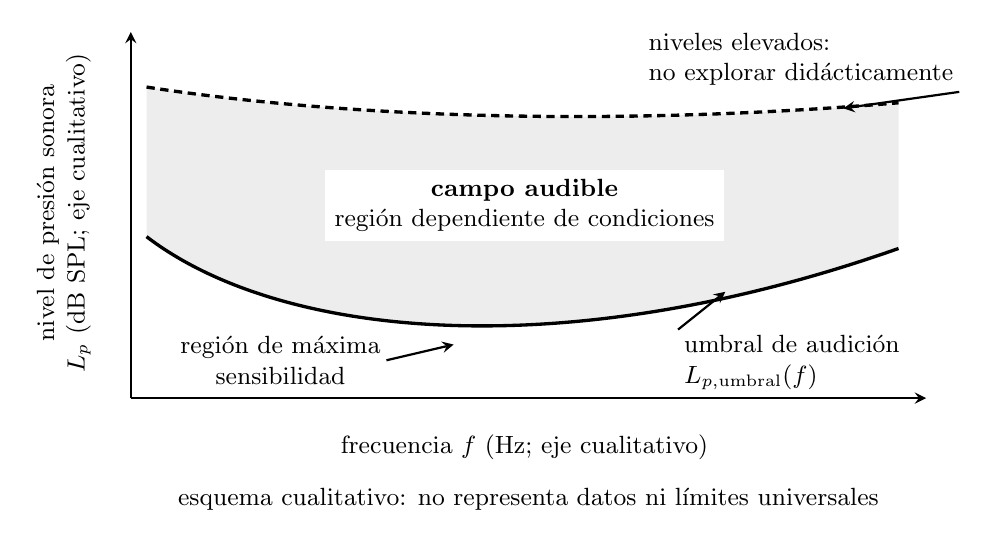
\begin{tikzpicture}[font=\small,>=stealth,x=1cm,y=1cm]
    \draw[->,thick] (1.10,0.80) -- (11.20,0.80);
    \draw[->,thick] (1.10,0.80) -- (1.10,5.45);
    \node at (6.10,0.18)
        {frecuencia \(f\) (Hz; eje cualitativo)};
    \node[rotate=90,align=center] at (0.25,3.15)
        {nivel de presión sonora\\\(L_p\) (dB SPL; eje cualitativo)};

    \path[fill=black!7]
        (1.30,2.85)
        .. controls (3.00,1.55) and (6.60,1.20) .. (10.85,2.70)
        -- (10.85,4.55)
        .. controls (7.30,4.25) and (3.90,4.35) .. (1.30,4.75)
        -- cycle;

    \draw[very thick]
        (1.30,2.85)
        .. controls (3.00,1.55) and (6.60,1.20) .. (10.85,2.70);
    \draw[very thick,densely dashed]
        (1.30,4.75)
        .. controls (3.90,4.35) and (7.30,4.25) .. (10.85,4.55);

    \node[fill=white,align=center] at (6.10,3.25)
        {\textbf{campo audible}\\
         región dependiente de condiciones};
    \node[anchor=west,align=left,fill=white,inner sep=2pt]
        (threshold-label) at (8.05,1.25)
        {umbral de audición\\
         \(L_{p,\mathrm{umbral}}(f)\)};
    \draw[->,thick]
        (threshold-label.north west) -- (8.65,2.15);

    \node[anchor=west,align=left,fill=white,inner sep=2pt]
        (upper-label) at (7.60,5.10)
        {niveles elevados:\\
         no explorar didácticamente};
    \draw[->,thick]
        (upper-label.south east) -- (10.15,4.48);

    \node[align=center,fill=white,inner sep=2pt]
        (sensitivity-label) at (3.00,1.28)
        {región de máxima\\sensibilidad};
    \draw[->,thick]
        (sensitivity-label.east) -- (5.20,1.48);

    \node[align=center] at (6.15,-0.48)
        {esquema cualitativo: no representa datos ni límites universales};
\end{tikzpicture}

    \caption{Lectura cualitativa del campo audible. La frontera inferior
    representa el umbral de audición para condiciones definidas y su región de
    menor nivel señala la máxima sensibilidad. La frontera superior recuerda
    que los niveles elevados no deben explorarse como actividad didáctica. Las
    curvas no proceden de mediciones ni fijan límites normativos; elaboración
    propia.}
    \label{fig:u7-umbral-campo-audible}
\end{figure}

\subsection{Campo libre, entrada del canal y tímpano}
\label{sec:u7-campo-timpano}

El nivel de presión sonora debe asociarse con una posición de medición. En un
ensayo de campo libre puede medirse el nivel en el punto donde estaría el
centro de la cabeza, pero sin el oyente. Cuando el oyente está presente, la
cabeza, el torso, el pabellón y el canal auditivo modifican la presión que
alcanza el tímpano.

Sean:

\begin{itemize}
    \item \(L_{p,\mathrm{campo}}(f)\), el nivel de presión sonora en el campo
    de referencia, expresado en \(\text{dB SPL}\);
    \item \(L_{p,\mathrm{T}}(f)\), el nivel próximo al tímpano,
    expresado en \(\text{dB SPL}\), donde el subíndice \(\mathrm{T}\)
    identifica esa posición;
    \item \(G_{\mathrm{CT}}(f)\), la diferencia de nivel entre ambas
    posiciones, expresada en decibeles (\(\text{dB}\)).
\end{itemize}

Se puede definir

\begin{equation}
    G_{\mathrm{CT}}(f)
      =L_{p,\mathrm{T}}(f)-L_{p,\mathrm{campo}}(f).
    \label{eq:u7-ganancia-campo-timpano}
\end{equation}

Esta diferencia es una respuesta de transferencia entre dos puntos y depende
de la frecuencia. No es un nivel absoluto en \(\text{dB SPL}\), no expresa
creación de energía y no equivale a una ganancia fija de sonoridad.

La transferencia campo--tímpano depende de la dirección de llegada,
la geometría individual y el punto exacto de medición. La resonancia del canal
auditivo y las contribuciones del pabellón y la concha participan en la mayor
sensibilidad de una región de frecuencias medias~\cite{carlini2024}. El modelo ideal de cuarto
de onda y sus limitaciones se presentaron en la
sección~\ref{sec:u6-modelo-cae}; aquí interesa su consecuencia perceptual, no
volver a derivar la anatomía.

La figura~\ref{fig:u7-campo-cae-timpano} permite comparar las dos posiciones
sin convertir su diferencia en un cambio fijo de sonoridad.

\begin{figure}[htbp]
    \centering
    % Propósito: distinguir el nivel medido en un punto de campo libre del nivel
% próximo al tímpano y mostrar que su diferencia es una transferencia
% dependiente de frecuencia, no una ganancia fija de sonoridad.
% Origen: G_CT(f)=L_p,T(f)-L_p,campo(f), ecuación
% \eqref{eq:u7-ganancia-campo-timpano}. Esquema geométrico sin escala.
% Descripción accesible: en el panel izquierdo una onda llega a un punto de
% referencia de campo libre sin oyente. En el panel derecho la misma onda llega
% a una cabeza esquemática; pabellón y canal conducen hacia el tímpano. Debajo
% se comparan los niveles en ambos puntos mediante la diferencia G_CT.
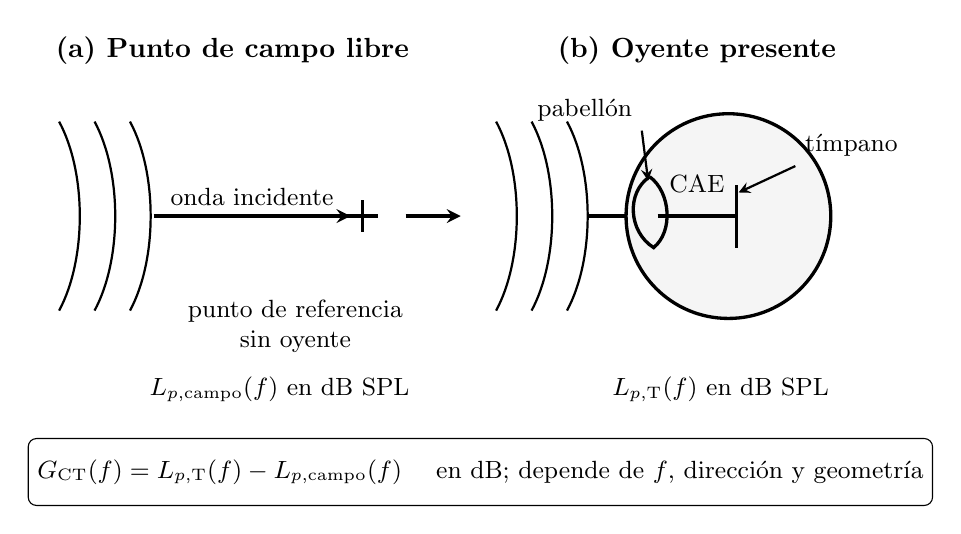
\begin{tikzpicture}[font=\small,>=stealth,x=1cm,y=1cm]
    \node[font=\bfseries] at (2.75,4.85)
        {(a) Punto de campo libre};
    \node[font=\bfseries] at (8.65,4.85)
        {(b) Oyente presente};

    % Panel (a).
    \foreach \xx in {0.55,1.00,1.45}{
        \draw[thick] (\xx,1.55) .. controls
            (\xx+0.35,2.20) and (\xx+0.35,3.30) .. (\xx,3.95);
    }
    \draw[->,very thick] (1.75,2.75) -- (4.25,2.75)
        node[midway,above] {onda incidente};
    \draw[very thick] (4.40,2.55) -- (4.40,2.95);
    \draw[very thick] (4.20,2.75) -- (4.60,2.75);
    \node[align=center] at (3.55,1.35)
        {punto de referencia\\sin oyente};
    \node[align=center] at (3.35,0.55)
        {\(L_{p,\mathrm{campo}}(f)\) en dB SPL};

    % Panel (b).
    \foreach \xx in {6.10,6.55,7.00}{
        \draw[thick] (\xx,1.55) .. controls
            (\xx+0.35,2.20) and (\xx+0.35,3.30) .. (\xx,3.95);
    }
    \draw[->,very thick] (7.25,2.75) -- (8.05,2.75);
    \draw[very thick,fill=black!4] (9.05,2.75) circle (1.30);
    \draw[very thick] (8.05,3.25)
        .. controls (7.75,3.05) and (7.78,2.55) .. (8.10,2.35)
        .. controls (8.35,2.55) and (8.32,3.05) .. (8.05,3.25);
    \draw[very thick] (8.15,2.75) -- (9.15,2.75);
    \draw[very thick] (9.15,2.35) -- (9.15,3.15);
    \node[anchor=east] (pinna-label) at (7.95,4.10) {pabellón};
    \draw[->,thick] (pinna-label.south east) -- (8.03,3.20);
    \node[anchor=south] at (8.65,2.92) {CAE};
    \node[anchor=west] (eardrum-label) at (9.90,3.65) {tímpano};
    \draw[->,thick] (eardrum-label.south west) -- (9.18,3.05);
    \node[align=center] at (8.95,0.55)
        {\(L_{p,\mathrm{T}}(f)\) en dB SPL};

    \draw[very thick,->] (4.95,2.75) -- (5.65,2.75);
    \node[align=center,draw,rounded corners=3pt,fill=white,
        minimum width=7.60cm,minimum height=0.85cm] at (5.90,-0.50)
        {\(\displaystyle
          G_{\mathrm{CT}}(f)
          =L_{p,\mathrm{T}}(f)-L_{p,\mathrm{campo}}(f)\)
         \quad en dB; depende de \(f\), dirección y geometría};
\end{tikzpicture}

    \caption{Nivel en un punto de campo libre frente a nivel próximo al
    tímpano. La presencia del oyente introduce una transferencia dependiente de
    frecuencia, dirección, geometría y posición de medición. La diferencia
    \(G_{\mathrm{CT}}\) se expresa en decibeles, pero no constituye un nivel
    absoluto ni una ganancia fija de sonoridad. Esquema sin escala; elaboración
    propia.}
    \label{fig:u7-campo-cae-timpano}
\end{figure}

\subsection{Ejemplo resuelto: dos posiciones de medición}
\label{sec:u7-ejemplo-campo-timpano}

En una situación didáctica se informan, para una misma frecuencia y bajo las
mismas condiciones, \(L_{p,\mathrm{campo}}=50\,\text{dB SPL}\) y
\(L_{p,\mathrm{T}}=58\,\text{dB SPL}\). Mediante la
ecuación~\eqref{eq:u7-ganancia-campo-timpano},

\[
    G_{\mathrm{CT}}
      =58\,\text{dB SPL}-50\,\text{dB SPL}
      =8\,\text{dB}.
\]

El resultado describe una diferencia entre posiciones para esa frecuencia.
No permite afirmar que la sonoridad aumentó una cantidad fija ni que todas las
personas presentan la misma transferencia.

\section{Curvas de igual sonoridad}
\label{sec:u7-isofonicas}

Una \textbf{curva de igual sonoridad} reúne combinaciones de frecuencia y
nivel de presión sonora que, bajo un procedimiento de comparación, producen
la misma sonoridad que un tono de referencia. También se la denomina
\textbf{curva isofónica}.

Las curvas normalizadas de igual sonoridad se obtienen para tonos
puros continuos, con condiciones de campo, dirección de incidencia, escucha y
población especificadas. La edición aplicable de la norma ISO 226 y sus datos
deben verificarse antes de incorporar una figura numérica~\cite{iso226_2023}. Fuera de esas
condiciones, las curvas constituyen una referencia y no una predicción exacta
para cualquier señal u oyente.

Las curvas permiten observar dos relaciones:

\begin{itemize}
    \item tonos de frecuencias diferentes pueden requerir niveles físicos
    diferentes para producir igual sonoridad;
    \item la separación entre curvas no permanece idéntica en todo el espectro
    ni para todos los niveles.
\end{itemize}

Por lo tanto, dos tonos con el mismo \(L_p\) no tienen por qué poseer igual
sonoridad. A la inversa, dos tonos juzgados igualmente sonoros no tienen por
qué compartir el mismo \(L_p\).

La figura~\ref{fig:isofonicas} muestra cómo los juicios de comparación producen
los puntos de una curva, sin sustituir los datos normalizados pendientes de
verificación.

\begin{figure}[htbp]
    \centering
    % Propósito: mostrar que una curva isofónica se construye mediante juicios de
% igual sonoridad bajo un procedimiento, no mediante igualdad de niveles.
% Origen: definición de curva de igual sonoridad de la sección
% \ref{sec:u7-isofonicas}. No se emplean datos de ISO 226 ni valores
% experimentales.
% Descripción accesible: tres bloques muestran un tono de referencia de
% 1000 Hz, un tono de prueba de frecuencia f cuyo nivel se ajusta y el juicio de
% igual sonoridad. A la derecha, un punto se incorpora a un plano de frecuencia
% y nivel; repetir el procedimiento para distintas frecuencias forma una curva.
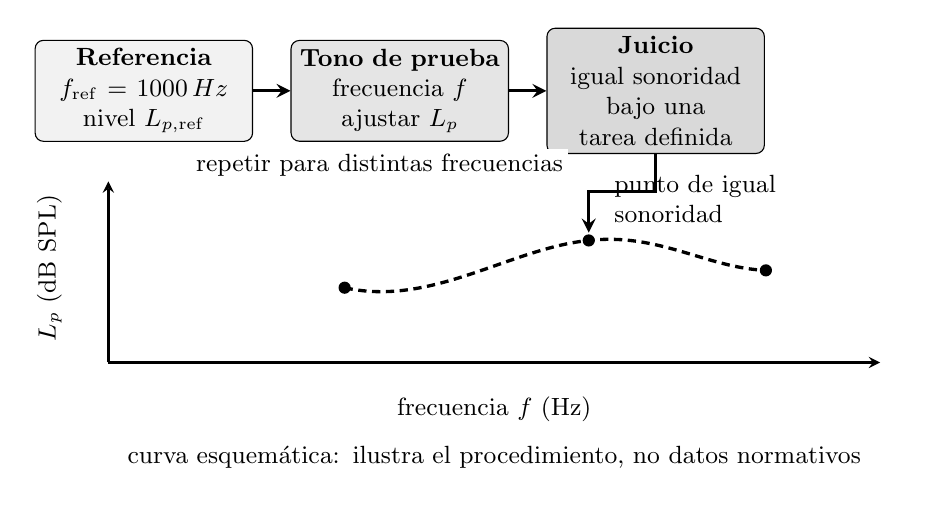
\begin{tikzpicture}[font=\small,>=stealth,x=1cm,y=1cm]
    \tikzset{
        stagebox/.style={draw,rounded corners=3pt,align=center,
            text width=2.55cm,minimum height=1.15cm,inner sep=3pt},
        flow/.style={->,very thick}
    }

    \node[stagebox,fill=black!5] (ref) at (1.55,4.00)
        {\textbf{Referencia}\\
         \(f_\mathrm{ref}=1000\,\text{Hz}\)\\
         nivel \(L_{p,\mathrm{ref}}\)};
    \node[stagebox,fill=black!10] (test) at (4.80,4.00)
        {\textbf{Tono de prueba}\\
         frecuencia \(f\)\\
         ajustar \(L_p\)};
    \node[stagebox,fill=black!15] (judge) at (8.05,4.00)
        {\textbf{Juicio}\\
         igual sonoridad\\
         bajo una tarea definida};

    \draw[flow] (ref.east) -- (test.west);
    \draw[flow] (test.east) -- (judge.west);

    \draw[->,thick] (1.10,0.55) -- (10.90,0.55);
    \draw[->,thick] (1.10,0.55) -- (1.10,2.85);
    \node at (6.00,-0.05) {frecuencia \(f\) (Hz)};
    \node[rotate=90] at (0.35,1.75) {\(L_p\) (dB SPL)};

    \fill (4.10,1.50) circle (2.2pt);
    \fill (7.20,2.10) circle (2.2pt);
    \fill (9.45,1.72) circle (2.2pt);
    \draw[very thick,densely dashed]
        (4.10,1.50) .. controls (5.20,1.25) and (6.20,2.00) ..
        (7.20,2.10) .. controls (8.10,2.20) and (8.70,1.75) ..
        (9.45,1.72);
    \node[anchor=west,align=left,fill=white,inner sep=2pt]
        at (7.45,2.63)
        {punto de igual\\sonoridad};

    \draw[flow] (judge.south) -- ++(0,-0.48) -| (7.20,2.20);
    \node[anchor=east,align=right,fill=white,inner sep=2pt]
        at (6.95,3.05)
        {repetir para distintas frecuencias};
    \node[align=center,text width=10.20cm] at (6.00,-0.65)
        {curva esquemática: ilustra el procedimiento, no datos normativos};
\end{tikzpicture}

    \caption{Construcción conceptual de una curva de igual sonoridad. Para cada
    frecuencia de prueba se ajusta el nivel hasta igualar la sonoridad de un
    tono de referencia bajo una tarea y condiciones definidas. La repetición
    aporta puntos de una curva isofónica. El trazado es esquemático y no
    reproduce datos de ISO~226; elaboración propia.}
    \label{fig:isofonicas}
\end{figure}

\section{Atributos perceptuales}
\label{sec:u7-atributos}

\subsection{Altura tonal o \emph{pitch}}
\label{sec:u7-pitch}

La \textbf{altura tonal} o \emph{pitch} es el atributo que permite ordenar
sensaciones desde más graves hasta más agudas. Para un tono puro sostenido y
bajo condiciones comparables, un aumento de frecuencia suele asociarse con un
aumento de altura tonal. Esta relación no convierte a frecuencia y
\emph{pitch} en sinónimos.

La altura tonal puede depender de periodicidad temporal, contenido
espectral, nivel, duración y contexto. En señales armónicas puede percibirse
una altura relacionada con la frecuencia fundamental aun cuando la componente
en esa frecuencia no esté presente~\cite{oxenham2018}. Este fenómeno de fundamental ausente
retoma la descripción espectral de la sección~\ref{sec:u5-componentes}: el
espectro físico no contiene una línea que el sistema auditivo ``agregue'', sino
que la altura emerge del patrón disponible.

\subsection{Sonoridad}
\label{sec:u7-sonoridad}

La \textbf{sonoridad} es el atributo perceptual que permite ordenar sonidos
desde menos sonoros hasta más sonoros. Suele aumentar cuando aumenta el nivel
de presión sonora, pero también depende de la frecuencia, la duración, el
ancho de banda, la distribución espectral, la presentación monoaural o
binaural y el contexto.

No debe afirmarse que una amplitud ``es el volumen''. La amplitud de presión
se mide en pascales (\(\text{Pa}\)); el nivel de presión sonora es una relación
física; la sonoridad es una respuesta perceptual. La palabra ``volumen'' puede
nombrar un control de ganancia de un equipo, pero no sustituye a ninguna de
esas magnitudes.

\subsection{Timbre}
\label{sec:u7-timbre}

El \textbf{timbre} permite diferenciar señales que pueden compartir altura
tonal, sonoridad y duración global. Participan la envolvente
espectral, la presencia de componentes armónicas o inarmónicas, el ruido, el
ataque, el decaimiento y otras variaciones temporales~\cite{oxenham2018}. Por eso, el timbre se
relaciona con el espectro, pero no se reduce a contar armónicos ni a observar
una única transformada de Fourier.

En una vocal sostenida, por ejemplo, la periodicidad de la fuente y la
envolvente asociada con las resonancias del tracto aportan informaciones
diferentes. Un análisis espectral ayuda a describir la señal, pero no mide por
sí solo el timbre percibido ni permite establecer un diagnóstico.

\subsection{Duración física y duración percibida}
\label{sec:u7-duracion}

La \textbf{duración física} \(\Delta t\) es el intervalo entre dos instantes y
se mide en segundos (\(\text{s}\)). La \textbf{duración percibida} es la
estimación temporal que realiza el oyente. Ambas se relacionan, pero la
respuesta también depende de los límites de la señal, el nivel, el espectro,
el contexto y la tarea.

Conviene separar tres nociones:

\begin{description}[style=nextline]
    \item[\textbf{Duración percibida:}]
    juicio sobre cuánto duró un evento.

    \item[\textbf{Resolución temporal:}]
    capacidad de distinguir cambios o separaciones en el tiempo.

    \item[\textbf{Integración temporal:}]
    efecto de acumular información de una señal durante un intervalo sobre la
    detección o la sonoridad.
\end{description}

Para estímulos breves, la detección y la sonoridad dependen de la
duración dentro de intervalos cuyo alcance varía con el estímulo y el
procedimiento~\cite{oxenham2018}. No corresponde reemplazar esa dependencia por un único
``umbral temporal'' aplicable a tonos, pausas y consonantes.

\section{Nivel de sonoridad y sonoridad: fones y sones}
\label{sec:u7-fones-sones}

El \textbf{nivel de sonoridad}, representado por \(L_N\), se expresa en fones
(\(\text{phon}\)). Su valor corresponde al nivel de presión sonora de
un tono de referencia de \(1000\,\text{Hz}\) que se juzga igualmente sonoro
bajo condiciones especificadas~\cite{asaPhon}. No se debe escribir ``un fon es un dB SPL'':
fon y dB SPL describen cantidades diferentes, aunque sus valores numéricos se
relacionen para el tono de referencia.

La \textbf{sonoridad}, representada por \(N\), se expresa en sones
(\(\text{sone}\)). La escala se define de modo que
\(1\,\text{sone}\) corresponda a \(40\,\text{phon}\) y una duplicación de
sonoridad corresponda a una duplicación del número de sones~\cite{asaSone}.

Para una conversión introductoria con niveles de sonoridad no menores
que \(40\,\text{phon}\), puede usarse~\cite{asaSone}

\begin{equation}
    N
      =2^{(L_N-40\,\text{phon})/(10\,\text{phon})}
        \,\text{sone},
    \label{eq:u7-fones-sones}
\end{equation}

donde \(L_N\) es el nivel de sonoridad en fones y \(N\) es la sonoridad en
sones. El exponente es adimensional porque se dividen cantidades expresadas en
la misma unidad.

La figura~\ref{fig:u7-fones-sones} representa la conversión del
modelo~\eqref{eq:u7-fones-sones} y permite reconocer que las dos cantidades
poseen unidades y escalas diferentes.

\begin{figure}[htbp]
    \centering
    % Propósito: enseñar que el nivel de sonoridad en fones y la sonoridad en sones
% son cantidades distintas, y visualizar la duplicación de sones cada 10 phon
% dentro del modelo introductorio.
% Origen: N=2^((L_N-40 phon)/(10 phon)) sone, ecuación
% \eqref{eq:u7-fones-sones}, para L_N>=40 phon. Valores calculados:
% 40, 50, 60, 70 y 80 phon corresponden a 1, 2, 4, 8 y 16 sone.
% Descripción accesible: un gráfico cartesiano muestra nivel de sonoridad entre
% 40 y 80 phon en el eje horizontal y sonoridad entre 0 y 16 sone en el
% vertical. La curva asciende de forma exponencial y pasa por cinco puntos
% rotulados; cada aumento de 10 phon duplica el número de sones.
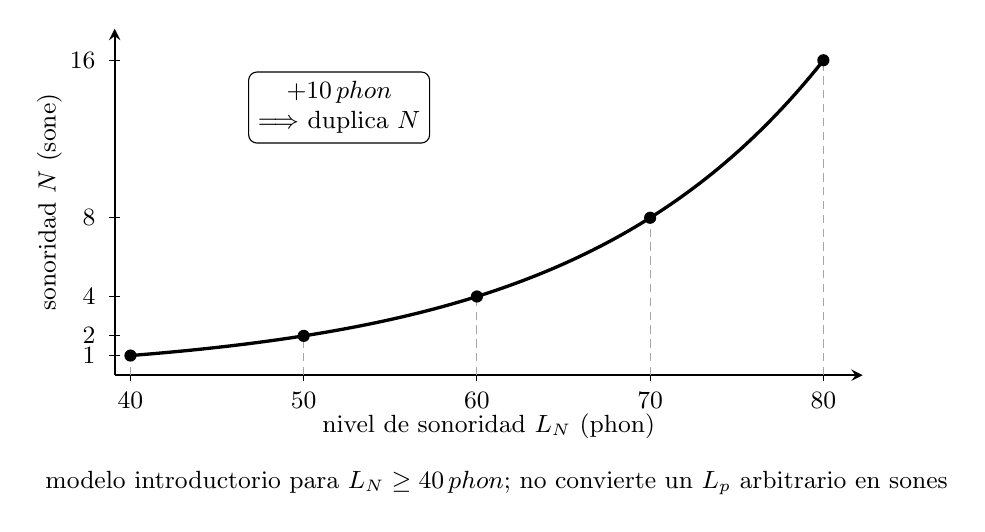
\begin{tikzpicture}[font=\small,>=stealth,x=1cm,y=1cm]
    \draw[->,thick] (1.15,0.75) -- (10.65,0.75);
    \draw[->,thick] (1.15,0.75) -- (1.15,5.15);
    \node at (5.90,0.10) {nivel de sonoridad \(L_N\) (phon)};
    \node[rotate=90] at (0.32,2.95) {sonoridad \(N\) (sone)};

    \foreach \ln/\x in {40/1.35,50/3.55,60/5.75,70/7.95,80/10.15}{
        \draw (\x,0.68) -- (\x,0.82);
        \node[anchor=north] at (\x,0.66) {\(\ln\)};
    }
    \foreach \n/\y in {1/1.00,2/1.25,4/1.75,8/2.75,16/4.75}{
        \draw (1.08,\y) -- (1.22,\y);
        \node[anchor=east] at (1.03,\y) {\(\n\)};
    }

    \draw[very thick,samples=100,domain=40:80]
        plot ({1.35+0.22*(\x-40)},
              {0.75+0.25*pow(2,(\x-40)/10)});

    \foreach \ln/\n/\x/\y in {
        40/1/1.35/1.00,
        50/2/3.55/1.25,
        60/4/5.75/1.75,
        70/8/7.95/2.75,
        80/16/10.15/4.75}{
        \draw[densely dashed,black!35] (\x,0.75) -- (\x,\y);
        \fill (\x,\y) circle (2.2pt);
    }

    \node[draw,rounded corners=3pt,fill=white,align=center] at (4.00,4.15)
        {\(+10\,\text{phon}\)\\
         \(\Longrightarrow\) duplica \(N\)};
    \node[align=center] at (6.00,-0.62)
        {modelo introductorio para \(L_N\geq40\,\text{phon}\);
         no convierte un \(L_p\) arbitrario en sones};
\end{tikzpicture}

    \caption{Relación entre nivel de sonoridad \(L_N\), expresado en fones, y
    sonoridad \(N\), expresada en sones, dentro del modelo introductorio de la
    ecuación~\eqref{eq:u7-fones-sones}. Cada aumento de
    \(10\,\text{phon}\) duplica el número de sones para
    \(L_N\geq40\,\text{phon}\). La gráfica no convierte un nivel de presión
    sonora arbitrario en sonoridad; elaboración propia.}
    \label{fig:u7-fones-sones}
\end{figure}

\subsection{Ejemplo resuelto: conversión acotada}
\label{sec:u7-ejemplo-sones}

Se informa un nivel de sonoridad \(L_N=70\,\text{phon}\). Dentro del modelo de
la ecuación~\eqref{eq:u7-fones-sones},

\[
    N
      =2^{(70\,\text{phon}-40\,\text{phon})/(10\,\text{phon})}
       \,\text{sone}
      =2^3\,\text{sone}
      =8\,\text{sone}.
\]

El resultado significa que la sonoridad representada por la escala es ocho
veces la referencia de \(1\,\text{sone}\). No significa que la intensidad
acústica sea ocho veces mayor. Tampoco autoriza a convertir directamente
\(70\,\text{dB SPL}\) en \(8\,\text{sone}\) para cualquier frecuencia o
señal.

\section{Enmascaramiento y filtros auditivos}
\label{sec:u7-enmascaramiento}

\subsection{Elevación del umbral}
\label{sec:u7-elevacion-umbral}

Existe \textbf{enmascaramiento} cuando la presencia de una señal
enmascarante modifica la detectabilidad de una señal objetivo. Para comparar
umbrales se definen:

\begin{itemize}
    \item \(L_{\mathrm{umbral,q}}(f_s)\), el nivel umbral de la señal objetivo
    en quietud, expresado en decibeles con una referencia declarada;
    \item \(L_{\mathrm{umbral,e}}(f_s)\), el nivel umbral en presencia del
    enmascarador, expresado con la misma referencia;
    \item \(M(f_s)\), la elevación del umbral o cantidad de enmascaramiento,
    expresada en decibeles (\(\text{dB}\));
    \item \(f_s\), la frecuencia de la señal objetivo, medida en
    \(\text{Hz}\).
\end{itemize}

La elevación del umbral se escribe

\begin{equation}
    M(f_s)
      =L_{\mathrm{umbral,e}}(f_s)
       -L_{\mathrm{umbral,q}}(f_s).
    \label{eq:u7-elevacion-umbral}
\end{equation}

El nivel del enmascarador no es igual, por definición, al umbral enmascarado.
La elevación depende de la relación espectral y temporal entre las señales,
sus niveles, duraciones y el procedimiento de detección.

\subsection{Enmascaramiento simultáneo}
\label{sec:u7-enmascaramiento-simultaneo}

En el \textbf{enmascaramiento simultáneo}, la señal objetivo y la señal
enmascarante se superponen al menos durante parte de su duración.
El enmascaramiento suele ser mayor cuando ambas producen excitación en
regiones auditivas próximas. Para determinados enmascaradores, el patrón de
elevación del umbral es asimétrico y puede extenderse más hacia frecuencias
superiores al aumentar el nivel~\cite{moore2008}.

Un \textbf{patrón de enmascaramiento} representa \(M(f_s)\) o el umbral
enmascarado en función de la frecuencia de la señal objetivo. Para
interpretarlo deben declararse el espectro y nivel del enmascarador, la
duración de ambas señales y el umbral en quietud.

\subsection{Filtros auditivos, banda crítica y ERB}
\label{sec:u7-filtros-auditivos}

Un modelo útil representa el análisis periférico mediante un banco de
\textbf{filtros auditivos} superpuestos. Cada filtro deja contribuir con mayor
peso a una región alrededor de su frecuencia central y con menor peso a
frecuencias alejadas.

La expresión \textbf{banda crítica} describe una región frecuencial relevante
para fenómenos como el enmascaramiento y la suma perceptual. La
\textbf{anchura rectangular equivalente} o ERB es una medida del ancho de un
filtro: corresponde al ancho de un filtro rectangular ideal con la misma
respuesta máxima y la misma área que el filtro considerado. Banda crítica y
ERB están relacionadas, pero no son nombres intercambiables de cualquier
intervalo de frecuencia.

Para estimar la ERB de filtros auditivos de oyentes jóvenes con
audición normal bajo las condiciones del modelo de Glasberg y Moore puede
utilizarse~\cite{glasbergMoore1990}

\begin{equation}
    \mathrm{ERB}_{N}(f_c)
      =24{,}7\,\text{Hz}
       \left(
       4{,}37\frac{f_c}{1000\,\text{Hz}}+1
       \right),
    \label{eq:u7-erb}
\end{equation}

donde \(f_c\) es la frecuencia central del filtro, medida en
\(\text{Hz}\), y \(\mathrm{ERB}_{N}\) se obtiene en \(\text{Hz}\). El
subíndice \(N\) recuerda que la aproximación no representa a cualquier oyente,
nivel o condición.

\subsection{Ejemplo resuelto: ERB estimada a 1000 Hz}
\label{sec:u7-ejemplo-erb}

Para \(f_c=1000\,\text{Hz}\),

\[
    \mathrm{ERB}_{N}
      =24{,}7\,\text{Hz}
       \left(
       4{,}37\frac{1000\,\text{Hz}}{1000\,\text{Hz}}+1
       \right)
      =132{,}639\,\text{Hz}
      \approx133\,\text{Hz}.
\]

El cociente de frecuencias es adimensional. El resultado es una estimación del
ancho equivalente del filtro dentro del modelo; no es el ancho obligatorio de
un ruido de enmascaramiento clínico.

La figura~\ref{fig:u7-enmascaramiento-erb} reúne dos lecturas que conviene no
confundir: la elevación de un umbral y la definición geométrica de la ERB.

\begin{figure}[htbp]
    \centering
    % Propósito: distinguir nivel del enmascarador, umbral enmascarado y elevación
% del umbral, y relacionar la selectividad de un filtro auditivo con su ERB.
% Origen: M(f_s)=L_umbral,e(f_s)-L_umbral,q(f_s), ecuación
% \eqref{eq:u7-elevacion-umbral}, y definición de ERB de la sección
% \ref{sec:u7-filtros-auditivos}. Curvas cualitativas; no son mediciones.
% Descripción accesible: el panel izquierdo muestra un umbral en quietud, un
% enmascarador y un umbral elevado; una flecha vertical marca M en la frecuencia
% de la señal objetivo. El panel derecho muestra la respuesta normalizada de un
% filtro y un rectángulo con la misma altura máxima y la misma área; su ancho es
% la ERB.
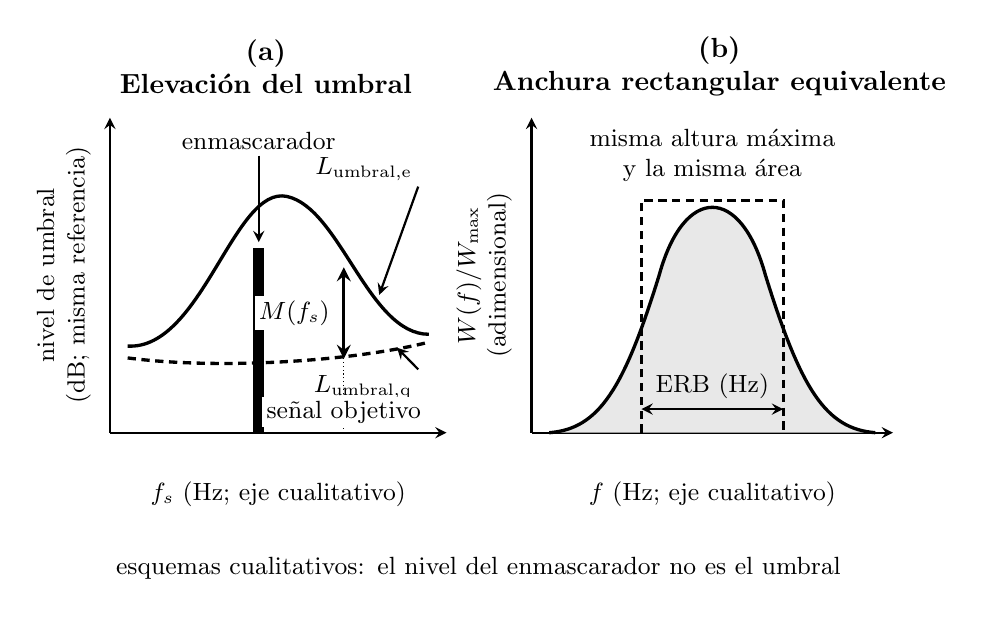
\begin{tikzpicture}[font=\small,>=stealth,x=0.90cm,y=1cm]
    \node[font=\bfseries,align=center] at (3.00,5.75)
        {(a)\\Elevación del umbral};
    \draw[->,thick] (0.80,1.10) -- (5.55,1.10)
        node[pos=0.50,below=14pt]
        {\(f_s\) (Hz; eje cualitativo)};
    \draw[->,thick] (0.80,1.10) -- (0.80,5.10);
    \node[rotate=90,align=center] at (0.15,3.10)
        {nivel de umbral\\(dB; misma referencia)};

    \draw[very thick,densely dashed]
        (1.05,2.05) .. controls (2.30,1.90) and (4.20,2.00) .. (5.30,2.25);
    \draw[very thick]
        (1.05,2.20) .. controls (2.10,2.15) and (2.55,4.25) ..
        (3.30,4.10) .. controls (4.05,3.95) and (4.45,2.35) ..
        (5.30,2.35);
    \draw[line width=4pt] (2.90,1.10) -- (2.90,3.45);
    \node[anchor=south,fill=white,inner sep=2pt]
        (masker-label) at (2.90,4.62) {enmascarador};
    \draw[->,thick] (masker-label.south) -- (2.90,3.52);

    \node[anchor=east,fill=white,inner sep=2pt]
        (masked-threshold-label) at (5.15,4.45)
        {\(L_{\mathrm{umbral,e}}\)};
    \draw[->,thick]
        (masked-threshold-label.south east) -- (4.60,2.85);
    \node[anchor=east,fill=white,inner sep=2pt]
        (quiet-threshold-label) at (5.15,1.68)
        {\(L_{\mathrm{umbral,q}}\)};
    \draw[->,thick]
        (quiet-threshold-label.north east) -- (4.85,2.18);

    \draw[densely dotted] (4.10,1.10) -- (4.10,3.20);
    \draw[<->,very thick] (4.10,2.04) -- (4.10,3.20)
        node[midway,left=3pt,fill=white,inner sep=1.5pt] {\(M(f_s)\)};
    \node[anchor=south,fill=white,inner sep=1.5pt]
        at (4.10,1.16) {señal objetivo};

    \node[font=\bfseries,align=center] at (9.40,5.75)
        {(b)\\Anchura rectangular equivalente};
    \draw[->,thick] (6.75,1.10) -- (11.85,1.10)
        node[pos=0.50,below=14pt]
        {\(f\) (Hz; eje cualitativo)};
    \draw[->,thick] (6.75,1.10) -- (6.75,5.10);
    \node[rotate=90,align=center] at (6.08,3.10)
        {\(W(f)/W_{\max}\)\\(adimensional)};

    \path[fill=black!9]
        (7.00,1.10)
        .. controls (7.70,1.15) and (8.05,1.65) .. (8.55,3.10)
        .. controls (8.90,4.25) and (9.70,4.25) .. (10.05,3.10)
        .. controls (10.55,1.65) and (10.90,1.15) .. (11.60,1.10)
        -- cycle;
    \draw[very thick]
        (7.00,1.10)
        .. controls (7.70,1.15) and (8.05,1.65) .. (8.55,3.10)
        .. controls (8.90,4.25) and (9.70,4.25) .. (10.05,3.10)
        .. controls (10.55,1.65) and (10.90,1.15) .. (11.60,1.10);

    \draw[very thick,densely dashed]
        (8.30,1.10) -- (8.30,4.05) -- (10.30,4.05) -- (10.30,1.10);
    \draw[<->,thick] (8.30,1.40) -- (10.30,1.40)
        node[midway,above] {\(\mathrm{ERB}\) (Hz)};
    \node[align=center] at (9.30,4.62)
        {misma altura máxima\\y la misma área};

    \node[align=center,text width=10.20cm] at (6.00,-0.62)
        {esquemas cualitativos: el nivel del enmascarador no es el umbral};
\end{tikzpicture}

    \caption{Enmascaramiento simultáneo y anchura rectangular equivalente.
    (a)~La elevación \(M(f_s)\) es la diferencia entre los umbrales en presencia
    del enmascarador y en quietud; el nivel del enmascarador no es el nuevo
    umbral. (b)~La ERB es el ancho de un rectángulo ideal con la misma altura
    máxima y la misma área que la respuesta del filtro considerado. Curvas
    cualitativas, no mediciones; elaboración propia.}
    \label{fig:u7-enmascaramiento-erb}
\end{figure}

\subsection{Enmascaramiento temporal}
\label{sec:u7-enmascaramiento-temporal}

El enmascaramiento también puede ocurrir sin superposición completa:

\begin{description}[style=nextline]
    \item[\textbf{Enmascaramiento hacia adelante:}]
    la señal enmascarante aparece antes que la señal objetivo y eleva
    transitoriamente su umbral.

    \item[\textbf{Enmascaramiento hacia atrás:}]
    la señal enmascarante aparece después que la señal objetivo y modifica su
    detectabilidad.
\end{description}

Sea \(\Delta t\) el intervalo entre el final de una señal y el comienzo de la
otra, medido en segundos (\(\text{s}\)). La elevación del umbral suele
disminuir cuando aumenta la separación temporal, pero la forma y el alcance de
esa disminución dependen del nivel, la duración, el espectro y la tarea. El
enmascaramiento hacia adelante suele ser más robusto que el enmascaramiento
hacia atrás~\cite{moore2008,bronkhorst2000}. No corresponde asignar una única ``ventana temporal'' válida
para cualquier señal.

La figura~\ref{fig:u7-enmascaramiento-temporal} muestra que los nombres hacia
adelante y hacia atrás se asignan por el orden de presentación respecto de la
señal objetivo.

\begin{figure}[htbp]
    \centering
    % Propósito: comparar simultaneidad, enmascaramiento hacia adelante y hacia
% atrás mediante el orden temporal de la señal objetivo y el enmascarador.
% Origen: definiciones de la sección
% \ref{sec:u7-enmascaramiento-temporal}. Duraciones y separaciones
% esquemáticas; no representan ventanas temporales universales.
% Descripción accesible: tres líneas de tiempo muestran, respectivamente,
% objetivo y enmascarador superpuestos, enmascarador antes del objetivo y
% objetivo antes del enmascarador. En los dos últimos casos una flecha marca la
% separación temporal Delta t.
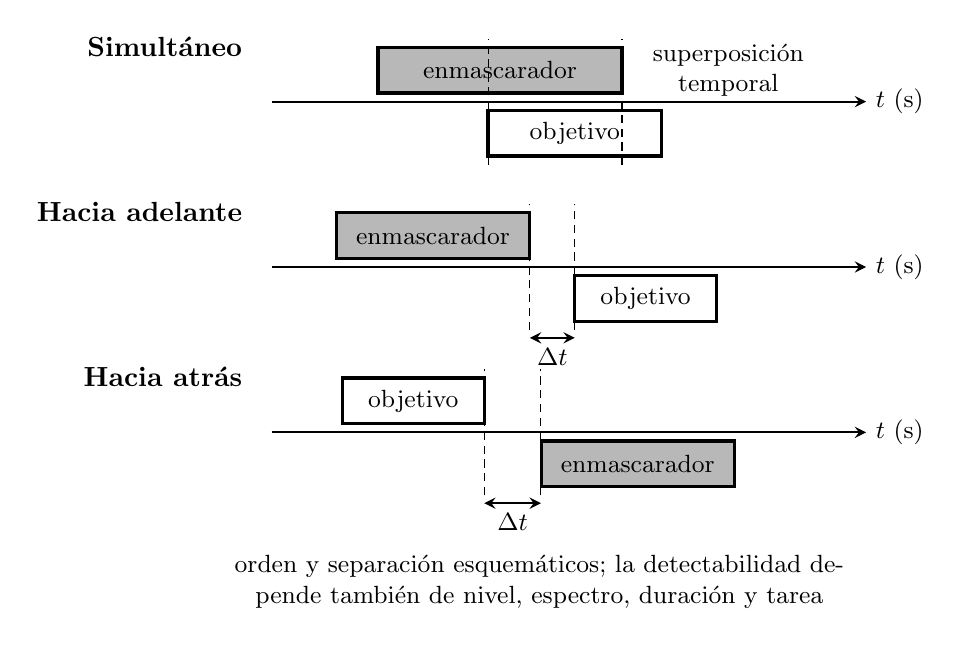
\begin{tikzpicture}[font=\small,>=stealth,x=1cm,y=1cm]
    \tikzset{
        masker/.style={draw,very thick,fill=black!28,minimum height=0.58cm},
        target/.style={draw,very thick,fill=white,minimum height=0.58cm}
    }

    \node[font=\bfseries,anchor=east] at (3.15,5.25) {Simultáneo};
    \draw[->,thick] (3.40,4.55) -- (10.95,4.55);
    \node[anchor=west] at (10.95,4.55) {\(t\) (s)};
    \node[masker,minimum width=3.10cm] at (6.30,4.95) {enmascarador};
    \node[target,minimum width=2.20cm] at (7.25,4.15) {objetivo};
    \draw[densely dashed] (6.15,3.75) -- (6.15,5.35);
    \draw[densely dashed] (7.85,3.75) -- (7.85,5.35);
    \node[align=center] at (9.20,4.95)
        {superposición\\temporal};

    \node[font=\bfseries,anchor=east] at (3.15,3.15)
        {Hacia adelante};
    \draw[->,thick] (3.40,2.45) -- (10.95,2.45);
    \node[anchor=west] at (10.95,2.45) {\(t\) (s)};
    \node[masker,minimum width=2.45cm] at (5.45,2.85) {enmascarador};
    \node[target,minimum width=1.80cm] at (8.15,2.05) {objetivo};
    \draw[densely dashed] (6.68,1.65) -- (6.68,3.25);
    \draw[densely dashed] (7.25,1.65) -- (7.25,3.25);
    \draw[<->,thick] (6.68,1.55) -- (7.25,1.55)
        node[midway,below] {\(\Delta t\)};

    \node[font=\bfseries,anchor=east] at (3.15,1.05)
        {Hacia atrás};
    \draw[->,thick] (3.40,0.35) -- (10.95,0.35);
    \node[anchor=west] at (10.95,0.35) {\(t\) (s)};
    \node[target,minimum width=1.80cm] at (5.20,0.75) {objetivo};
    \node[masker,minimum width=2.45cm] at (8.05,-0.05) {enmascarador};
    \draw[densely dashed] (6.10,-0.45) -- (6.10,1.15);
    \draw[densely dashed] (6.82,-0.45) -- (6.82,1.15);
    \draw[<->,thick] (6.10,-0.55) -- (6.82,-0.55)
        node[midway,below] {\(\Delta t\)};

    \node[align=center,text width=9.70cm] at (6.80,-1.55)
        {orden y separación esquemáticos; la detectabilidad depende también
         de nivel, espectro, duración y tarea};
\end{tikzpicture}

    \caption{Relaciones temporales entre señal objetivo y enmascarador. En el
    enmascaramiento simultáneo existe superposición; hacia adelante, el
    enmascarador precede al objetivo; hacia atrás, lo sigue. Las duraciones y
    separaciones son esquemáticas y no representan una ventana temporal
    universal; elaboración propia.}
    \label{fig:u7-enmascaramiento-temporal}
\end{figure}

\subsection{Enmascaramiento energético e informacional}
\label{sec:u7-enmascaramiento-energetico-informacional}

El \textbf{enmascaramiento energético} se relaciona con la superposición de
energía del objetivo y del enmascarador dentro de los filtros auditivos y con
la reducción de las pistas periféricas disponibles.

El \textbf{enmascaramiento informacional} describe dificultades adicionales
para seleccionar, organizar o identificar la fuente objetivo aun cuando la
superposición energética no explique por completo el desempeño.
La semejanza entre voces, la incertidumbre sobre la fuente y la
competencia por la atención pueden contribuir al enmascaramiento
informacional~\cite{moore2008,bronkhorst2000}.

La distinción es conceptual: en una escena real pueden coexistir ambos
componentes. La Unidad~\ref{chap:unidad-10} describirá las propiedades físicas de ruidos
blancos, rosas, vocales y de banda estrecha, además de su aplicación
audiométrica introductoria, sin repetir este mecanismo perceptual.

\section{Voz, reverberación e inteligibilidad}
\label{sec:u7-inteligibilidad}

\subsection{Relación señal--ruido}
\label{sec:u7-snr}

La \textbf{inteligibilidad del habla} es el grado en que un oyente identifica
correctamente unidades lingüísticas bajo una tarea definida. Puede evaluarse
con fonemas, sílabas, palabras u oraciones, por lo que un porcentaje solo puede
interpretarse si se conocen el material, la lengua, el procedimiento y la
población.

Para una descripción física introductoria pueden compararse el nivel de la
señal de habla \(L_{p,\mathrm{s}}\) y el nivel del ruido
\(L_{p,\mathrm{n}}\), ambos expresados en \(\text{dB SPL}\), medidos con la
misma ponderación, ancho de banda, posición e intervalo. La relación
señal--ruido se expresa como

\begin{equation}
    \mathrm{SNR}
      =L_{p,\mathrm{s}}-L_{p,\mathrm{n}},
    \label{eq:u7-snr}
\end{equation}

y se informa en decibeles (\(\text{dB}\)). Una SNR mayor suele favorecer la
disponibilidad física de pistas del habla, pero no determina por sí sola un
porcentaje de inteligibilidad.

\subsection{Reverberación y reflexiones tardías}
\label{sec:u7-reverberacion}

La reverberación se origina por reflexiones sucesivas y se caracterizará
físicamente en la Unidad~\ref{chap:unidad-9}. Desde la percepción importa que
parte de la energía
de un segmento persiste y se superpone con segmentos posteriores.

Una reverberación excesiva puede reducir contrastes temporales y
espectrales del habla, y su efecto suele combinarse con el ruido de fondo. La
inteligibilidad depende también de la distancia, la directividad, el material
lingüístico y las características del oyente~\cite{moore2008,moser2009}. Por eso, no existe una ecuación
lineal universal que convierta SNR y tiempo de reverberación en porcentaje de
palabras comprendidas.

El índice de transmisión del habla (STI) y el índice de
inteligibilidad del habla (SII) son métodos diferentes, con entradas, supuestos
y dominios propios~\cite{iec60268_16_2020}. En esta unidad basta reconocer qué problema intentan
representar; su cálculo normativo requiere fuentes y procedimientos que
exceden el alcance introductorio.

\subsection{Pérdida de articulación de consonantes}
\label{sec:u7-alcons}

La \textbf{pérdida de articulación de consonantes} expresa el porcentaje de
consonantes presentadas que no fueron identificadas correctamente en una
prueba definida. Sean \(n_\mathrm{p}\), la cantidad de consonantes
presentadas, y \(n_\mathrm{c}\), la cantidad identificada correctamente; ambas
son conteos adimensionales. Entonces,

\begin{equation}
    \mathrm{ALCons}
      =100\left(1-\frac{n_\mathrm{c}}{n_\mathrm{p}}\right)\%.
    \label{eq:u7-alcons}
\end{equation}

Esta ecuación calcula un porcentaje observado; no predice por sí sola el
resultado de otra sala o población. Los modelos que estiman ALCons a
partir de variables acústicas poseen condiciones de validez y no deben
aplicarse sin verificar la definición del ensayo, el campo sonoro y la fuente
bibliográfica~\cite{iec60268_16_2020,moser2009}.

\subsection{Ejemplo resuelto: porcentaje observado}
\label{sec:u7-ejemplo-alcons}

En una actividad didáctica se presentan \(n_\mathrm{p}=80\) consonantes y se
identifican correctamente \(n_\mathrm{c}=68\). Mediante la
ecuación~\eqref{eq:u7-alcons},

\[
    \mathrm{ALCons}
      =100\left(1-\frac{68}{80}\right)\%
      =15\%.
\]

El resultado describe solamente esa actividad. No permite atribuir el error a
ruido, reverberación o audición sin comparar condiciones y conocer el
procedimiento.

\section{Percepción de reflexiones y efecto de precedencia}
\label{sec:u7-precedencia}

Cuando una señal directa y una reflexión alcanzan al oyente, la reflexión
posee un recorrido adicional. Sean \(\Delta r\), la diferencia de recorrido,
medida en metros (\(\text{m}\)); \(c\), la velocidad de propagación, medida en
metros por segundo (\(\text{m}/\text{s}\)); y \(\Delta t\), el retardo,
medido en segundos (\(\text{s}\)). En un medio aproximadamente uniforme,

\begin{equation}
    \Delta t=\frac{\Delta r}{c}.
    \label{eq:u7-retardo-reflexion}
\end{equation}

El retardo físico no determina por sí solo qué se percibe. También importan la
diferencia de nivel, la duración, el espectro, la dirección de llegada, la
repetición y el ambiente.

El \textbf{efecto de precedencia} reúne al menos tres observaciones
relacionadas: la fusión de eventos próximos, el predominio de la primera
llegada en la localización y la menor capacidad para discriminar cambios en la
llegada posterior. Estas observaciones no comparten necesariamente un único
límite temporal~\cite{litovsky1999}.

El término \textbf{efecto Haas} se reserva aquí para el resultado histórico
obtenido con habla y una repetición retardada, relacionado con audibilidad,
localización e inteligibilidad. No se lo utilizará como sinónimo de todos los
fenómenos de precedencia.

Al variar el retardo y el nivel de una reflexión pueden observarse
coloración, aumento de extensión o sonoridad, desplazamientos espaciales,
fusión y, para ciertas condiciones, una repetición separada o eco~\cite{litovsky1999}. La
transición es gradual y dependiente del estímulo; por eso no corresponde
prescribir un retardo universal para sistemas de refuerzo sonoro.

La figura~\ref{fig:u7-precedencia-reflexiones} separa el cálculo geométrico del
retardo de la interpretación perceptual de las dos llegadas.

\begin{figure}[htbp]
    \centering
    % Propósito: relacionar el recorrido adicional de una reflexión con su retardo
% y evitar interpretar ese retardo como un umbral perceptual universal.
% Origen: Delta t=Delta r/c, ecuación
% \eqref{eq:u7-retardo-reflexion}, y discusión de la sección
% \ref{sec:u7-precedencia}. Geometría esquemática sin escala.
% Descripción accesible: el panel izquierdo muestra una fuente, un oyente y una
% pared; una flecha recta representa la llegada directa y otra, más larga,
% rebota en la pared. El panel derecho muestra dos llegadas sobre un eje
% temporal separadas por Delta t. Una nota indica que la percepción depende de
% otras propiedades además del retardo.
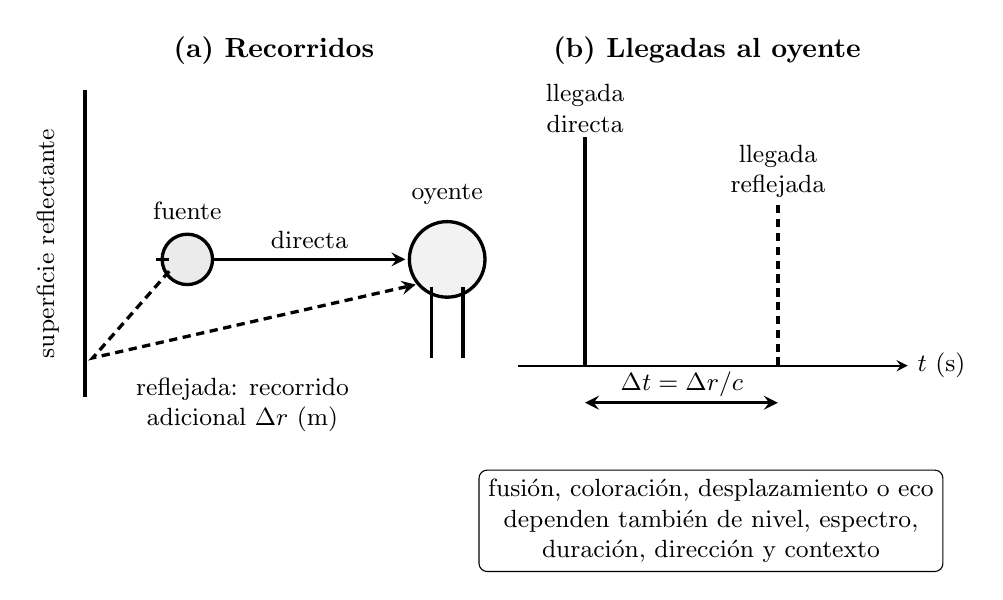
\begin{tikzpicture}[font=\small,>=stealth,x=1cm,y=1cm]
    \node[font=\bfseries] at (3.15,5.25)
        {(a) Recorridos};
    \draw[very thick] (0.75,0.85) -- (0.75,4.75);
    \node[rotate=90] at (0.28,2.80) {superficie reflectante};

    \draw[very thick,fill=black!8] (2.05,2.60) circle (0.32);
    \draw[very thick] (1.65,2.60) -- (1.82,2.60);
    \node[anchor=south] at (2.05,2.98) {fuente};

    \draw[very thick,fill=black!5] (5.35,2.60) circle (0.48);
    \draw[very thick] (5.15,2.25) -- (5.15,1.35);
    \draw[very thick] (5.55,2.25) -- (5.55,1.35);
    \node[anchor=south] at (5.35,3.18) {oyente};

    \draw[->,very thick] (2.38,2.60) -- (4.82,2.60)
        node[midway,above] {directa};
    \draw[->,very thick,densely dashed]
        (1.82,2.45) -- (0.85,1.35) -- (4.95,2.28);
    \node[align=center] at (2.75,0.75)
        {reflejada: recorrido\\adicional \(\Delta r\) (m)};

    \node[font=\bfseries] at (8.65,5.25)
        {(b) Llegadas al oyente};
    \draw[->,thick] (6.25,1.25) -- (11.20,1.25);
    \node[anchor=west] at (11.20,1.25) {\(t\) (s)};
    \draw[very thick] (7.10,1.25) -- (7.10,4.15);
    \draw[very thick,densely dashed] (9.55,1.25) -- (9.55,3.35);
    \node[align=center] at (7.10,4.52) {llegada\\directa};
    \node[align=center] at (9.55,3.72) {llegada\\reflejada};
    \draw[<->,very thick] (7.10,0.78) -- (9.55,0.78);
    \node[fill=white,inner sep=1.5pt] at (8.33,1.02)
        {\(\Delta t=\Delta r/c\)};

    \node[draw,rounded corners=3pt,align=center,fill=white,
        minimum width=4.50cm] at (8.70,-0.72)
        {fusión, coloración, desplazamiento o eco\\
         dependen también de nivel, espectro,\\
         duración, dirección y contexto};
\end{tikzpicture}

    \caption{Señal directa y reflexión. El recorrido adicional
    \(\Delta r\) produce el retardo físico
    \(\Delta t=\Delta r/c\). La posición relativa de las llegadas puede
    calcularse, pero la percepción de fusión, coloración, desplazamiento o eco
    depende además de nivel, espectro, duración, dirección y contexto. Esquema
    sin escala; elaboración propia.}
    \label{fig:u7-precedencia-reflexiones}
\end{figure}

\subsection{Ejemplo resuelto: retardo geométrico}
\label{sec:u7-ejemplo-reflexion}

Una reflexión recorre \(\Delta r=3{,}43\,\text{m}\) adicionales respecto de
la señal directa. Si se adopta \(c=343\,\text{m}/\text{s}\),

\[
    \Delta t
      =\frac{3{,}43\,\text{m}}{343\,\text{m}/\text{s}}
      =0{,}0100\,\text{s}
      =10{,}0\,\text{ms}.
\]

El cálculo informa el retardo físico. Para anticipar la percepción todavía
sería necesario conocer nivel, espectro, duración, dirección y contexto.

\section{Audición espacial}
\label{sec:u7-audicion-espacial}

\subsection{Audición binaural, ITD e ILD}
\label{sec:u7-itd-ild}

La audición \textbf{binaural} utiliza información que resulta de comparar las
señales disponibles en ambos oídos. Dos pistas centrales son:

\begin{description}[style=nextline]
    \item[\textbf{Diferencia interaural de tiempo (ITD):}]
    diferencia entre los tiempos de llegada o entre estructuras temporales de
    las señales de ambos oídos. Se representa mediante
    \(\Delta t_\mathrm{LR}\) y se mide en segundos (\(\text{s}\)).

    \item[\textbf{Diferencia interaural de nivel (ILD):}]
    diferencia entre niveles comparables en el oído izquierdo y el derecho.
    Si \(L_{p,\mathrm{L}}\) y \(L_{p,\mathrm{R}}\) son niveles expresados en
    \(\text{dB SPL}\), se puede escribir
    \[
        \mathrm{ILD}=L_{p,\mathrm{L}}-L_{p,\mathrm{R}},
    \]
    y el resultado se expresa en decibeles (\(\text{dB}\)).
\end{description}

Para muchas señales, las ITD aportan información especialmente útil
en bajas frecuencias y las ILD adquieren mayor importancia cuando la sombra
acústica de la cabeza es apreciable. La utilidad de cada pista depende de
frecuencia, ancho de banda, envolvente temporal, dirección y geometría, por lo
que no existe una frontera única que separe ambos mecanismos~\cite{carlini2024}.

\subsection{Modelo geométrico de ITD}
\label{sec:u7-modelo-itd}

Un modelo inicial ignora la difracción alrededor de la cabeza y aproxima la
máxima diferencia de recorrido mediante una distancia interaural efectiva
\(d\), medida en metros (\(\text{m}\)). Si \(c\) es la velocidad de
propagación en \(\text{m}/\text{s}\), entonces

\begin{equation}
    \lvert\Delta t_\mathrm{LR}\rvert
      \approx\frac{d}{c}.
    \label{eq:u7-itd-geometrica}
\end{equation}

Para un valor didáctico \(d=0{,}180\,\text{m}\) y
\(c=343\,\text{m}/\text{s}\),

\[
    \lvert\Delta t_\mathrm{LR}\rvert
      \approx\frac{0{,}180\,\text{m}}{343\,\text{m}/\text{s}}
      \approx5{,}25\times10^{-4}\,\text{s}
      =0{,}525\,\text{ms}.
\]

El resultado es un orden de magnitud del modelo rectilíneo. No representa una
constante anatómica ni reemplaza un modelo de propagación alrededor de la
cabeza.

\subsection{Pistas espectrales y cono de confusión}
\label{sec:u7-pistas-espectrales}

La cabeza, el torso y los pabellones producen modificaciones dependientes de
frecuencia y dirección. Estas modificaciones se describen mediante funciones
de transferencia relacionadas con la cabeza y aportan
\textbf{pistas espectrales}.

Distintas posiciones pueden producir ITD e ILD semejantes y formar un
cono de confusión. Las pistas espectrales, la familiaridad con la respuesta
propia y los movimientos de la cabeza ayudan a resolver ambigüedades
arriba--abajo y adelante--atrás~\cite{carlini2024}. Por eso, la localización no puede explicarse
solo mediante dos números interaurales.

La figura~\ref{fig:u7-localizacion} integra las pistas interaurales con las
pistas espectrales y dinámicas que reducen ambigüedades.

\begin{figure}[htbp]
    \centering
    % Propósito: integrar ITD, ILD y pistas espectrales, y mostrar por qué dos
% números interaurales no resuelven por sí solos todas las posiciones.
% Origen: definiciones de ITD e ILD, modelo
% \eqref{eq:u7-itd-geometrica} y discusión del cono de confusión de las
% secciones \ref{sec:u7-itd-ild}--\ref{sec:u7-pistas-espectrales}.
% Geometría conceptual sin escala ni valores anatómicos.
% Descripción accesible: el panel izquierdo muestra una fuente lateral y dos
% recorridos hacia los oídos; el oído cercano recibe antes y con otro nivel. El
% panel derecho muestra dos fuentes sobre un arco de posiciones que podrían
% compartir ITD e ILD; pabellón y movimiento de cabeza aportan pistas
% espectrales y dinámicas para reducir la ambigüedad.
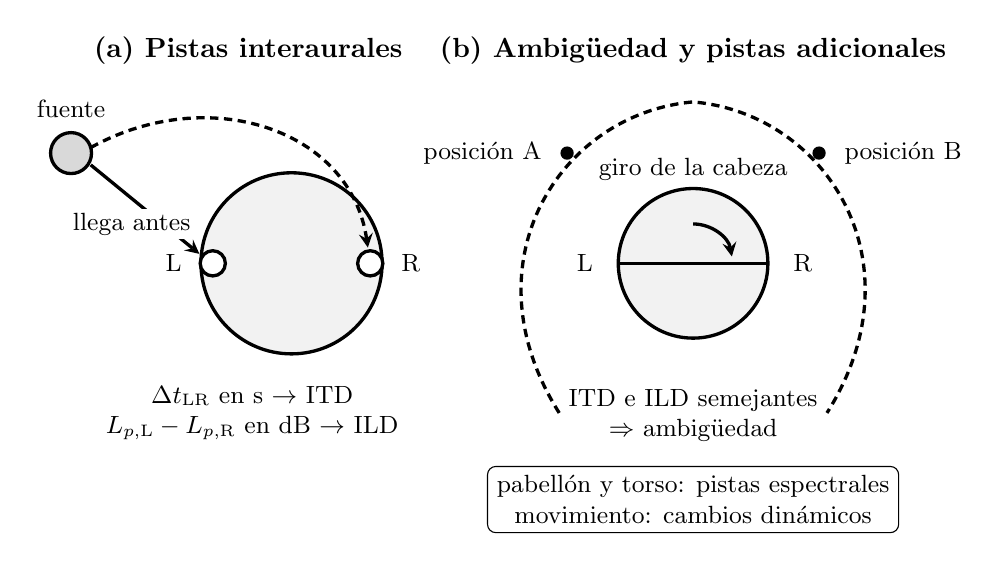
\begin{tikzpicture}[font=\small,>=stealth,x=1cm,y=1cm]
    \node[font=\bfseries] at (3.10,5.45)
        {(a) Pistas interaurales};
    \draw[very thick,fill=black!5] (3.65,2.75) circle (1.15);
    \draw[very thick,fill=white] (2.65,2.75) circle (0.16);
    \draw[very thick,fill=white] (4.65,2.75) circle (0.16);
    \node[anchor=east] at (2.38,2.75) {L};
    \node[anchor=west] at (4.92,2.75) {R};

    \draw[very thick,fill=black!15] (0.85,4.15) circle (0.26);
    \node[anchor=south] at (0.85,4.48) {fuente};
    \draw[->,very thick] (1.10,4.00) -- (2.48,2.87);
    \node[fill=white,inner sep=1.5pt] at (1.62,3.25)
        {llega antes};
    \draw[->,very thick,densely dashed]
        (1.10,4.22) .. controls (2.60,5.05) and (4.40,4.45) .. (4.62,2.95);
    \node[align=center] at (3.15,0.85)
        {\(\Delta t_\mathrm{LR}\) en s \(\rightarrow\) ITD\\
         \(L_{p,\mathrm{L}}-L_{p,\mathrm{R}}\) en dB \(\rightarrow\) ILD};

    \node[font=\bfseries] at (8.75,5.45)
        {(b) Ambigüedad y pistas adicionales};
    \draw[very thick,fill=black!5] (8.75,2.75) circle (0.95);
    \draw[very thick] (7.80,2.75) -- (9.70,2.75);
    \node[anchor=east] at (7.60,2.75) {L};
    \node[anchor=west] at (9.90,2.75) {R};

    \draw[very thick,densely dashed]
        (7.05,0.85) .. controls (5.85,2.75) and (7.05,4.65) ..
        (8.75,4.80) .. controls (10.45,4.65) and (11.65,2.75) ..
        (10.45,0.85);
    \fill (7.15,4.15) circle (2.4pt);
    \fill (10.35,4.15) circle (2.4pt);
    \node[anchor=east,align=right] at (6.95,4.15)
        {posición A};
    \node[anchor=west,align=left] at (10.55,4.15)
        {posición B};
    \node[align=center] at (8.75,0.82)
        {ITD e ILD semejantes\\
         \(\Rightarrow\) ambigüedad};

    \draw[->,very thick]
        (8.75,3.25) arc[start angle=90,end angle=10,radius=0.50];
    \node[align=center,fill=white,inner sep=1.5pt] at (8.75,3.95)
        {giro de la cabeza};
    \node[draw,rounded corners=3pt,align=center,fill=white] at (8.75,-0.25)
        {pabellón y torso: pistas espectrales\\
         movimiento: cambios dinámicos};
\end{tikzpicture}

    \caption{Pistas para la audición espacial. (a)~Una fuente lateral puede
    producir diferencias interaurales de tiempo y nivel. (b)~Posiciones
    distintas pueden compartir ITD e ILD semejantes; las modificaciones
    espectrales del pabellón, la cabeza y el torso, junto con el movimiento,
    aportan información adicional. Geometría conceptual sin escala;
    elaboración propia.}
    \label{fig:u7-localizacion}
\end{figure}

\section{Escucha con fuentes concurrentes}
\label{sec:u7-cocktail-party}

En una conversación con varias fuentes, el sistema auditivo debe organizar la
mezcla en objetos o corrientes perceptuales y seleccionar la voz objetivo. El
llamado \textbf{efecto \emph{cocktail party}} no es un filtro físico único,
sino una situación en la que intervienen:

\begin{itemize}
    \item separación espacial y pistas binaurales;
    \item diferencias de altura tonal, timbre y evolución temporal;
    \item continuidad y coherencia de cada fuente;
    \item atención, expectativas y conocimiento del mensaje;
    \item enmascaramiento energético e informacional.
\end{itemize}

Separar espacialmente la voz objetivo y las voces competidoras puede
producir liberación espacial del enmascaramiento. El beneficio depende de la
escena, del oyente y del acceso a las pistas binaurales~\cite{bronkhorst2000}. Un micrófono
direccional puede modificar la SNR física que llega a un dispositivo, pero ese
cambio no debe confundirse con el mecanismo perceptual completo ni presentarse
como una mejora fija de inteligibilidad.

La figura~\ref{fig:u7-fuentes-concurrentes} resume la escena sin representar el
efecto \emph{cocktail party} como un filtro físico único.

\begin{figure}[htbp]
    \centering
    % Propósito: integrar las pistas físicas y perceptuales que intervienen al
% seleccionar una voz entre fuentes concurrentes, evitando representar el
% efecto cocktail party como un filtro físico único.
% Origen: factores enumerados en la sección
% \ref{sec:u7-cocktail-party}. Escena conceptual sin datos ni resultado
% clínico.
% Descripción accesible: una persona escucha una voz objetivo situada al
% frente, dos voces competidoras a los lados y ruido de ventilación detrás. Las
% flechas llegan a ambos oídos. Un bloque lateral separa pistas físicas como
% SNR y dirección de procesos perceptuales como segregación y atención.
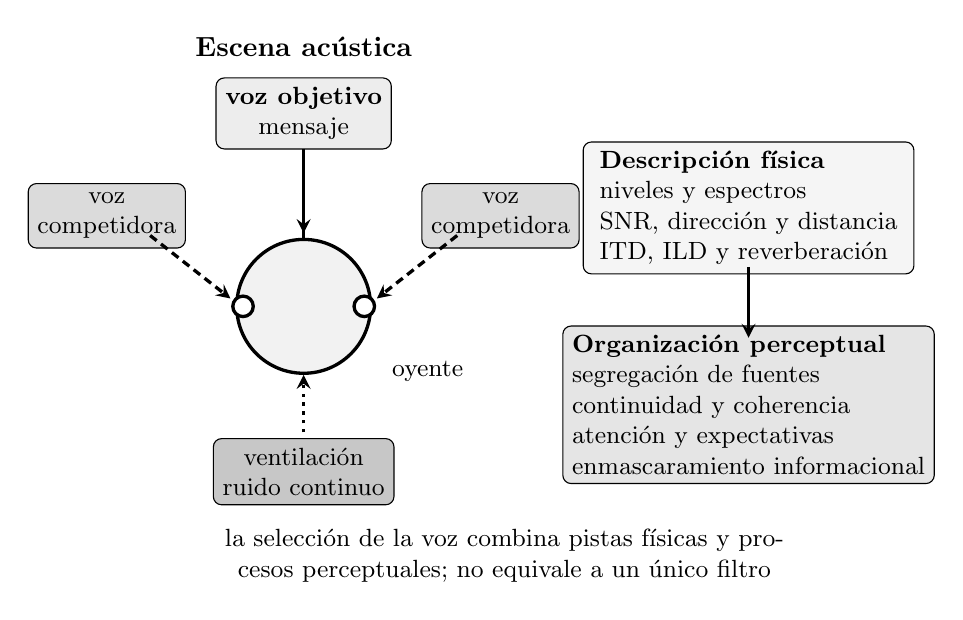
\begin{tikzpicture}[font=\small,>=stealth,x=1cm,y=1cm]
    \node[font=\bfseries] at (3.45,5.85)
        {Escena acústica};

    \draw[very thick,fill=black!5] (3.45,2.55) circle (0.85);
    \draw[very thick,fill=white] (2.68,2.55) circle (0.13);
    \draw[very thick,fill=white] (4.22,2.55) circle (0.13);
    \draw[very thick] (3.45,3.40) -- (3.45,3.82);
    \node[anchor=west] at (4.45,1.72) {oyente};

    \node[draw,rounded corners=3pt,fill=black!7,align=center] at (3.45,5.00)
        {\textbf{voz objetivo}\\mensaje};
    \node[draw,rounded corners=3pt,fill=black!14,align=center] at (0.95,3.70)
        {voz\\competidora};
    \node[draw,rounded corners=3pt,fill=black!14,align=center] at (5.95,3.70)
        {voz\\competidora};
    \node[draw,rounded corners=3pt,fill=black!22,align=center] at (3.45,0.45)
        {ventilación\\ruido continuo};

    \draw[->,very thick] (3.45,4.55) -- (3.45,3.48);
    \draw[->,very thick,densely dashed]
        (1.50,3.45) -- (2.52,2.65);
    \draw[->,very thick,densely dashed]
        (5.40,3.45) -- (4.38,2.65);
    \draw[->,very thick,dotted] (3.45,0.95) -- (3.45,1.68);

    \node[draw,rounded corners=3pt,align=left,minimum width=4.20cm,
        fill=black!4] at (9.10,3.80)
        {\textbf{Descripción física}\\
         niveles y espectros\\
         SNR, dirección y distancia\\
         ITD, ILD y reverberación};
    \node[draw,rounded corners=3pt,align=left,minimum width=4.20cm,
        fill=black!10] at (9.10,1.30)
        {\textbf{Organización perceptual}\\
         segregación de fuentes\\
         continuidad y coherencia\\
         atención y expectativas\\
         enmascaramiento informacional};
    \draw[->,very thick] (9.10,3.05) -- (9.10,2.15);

    \node[align=center,text width=10.20cm] at (6.00,-0.62)
        {la selección de la voz combina pistas físicas y procesos perceptuales;
         no equivale a un único filtro};
\end{tikzpicture}

    \caption{Escucha con fuentes concurrentes. La mezcla física contiene una
    voz objetivo, voces competidoras, ruido y reflexiones; puede describirse
    mediante niveles, espectros, SNR y dirección. La selección perceptual
    combina esas pistas con segregación, continuidad, atención y
    enmascaramiento informacional. Escena conceptual sin escala; elaboración
    propia.}
    \label{fig:u7-fuentes-concurrentes}
\end{figure}
\section{Relación con Fonoaudiología}
\label{sec:u7-relacion-fonoaudiologia}

Los conceptos de esta unidad ayudan a formular preguntas físicamente
precisas:

\begin{itemize}
    \item una diferencia en \(\text{dB SPL}\) no informa por sí sola una
    diferencia de sonoridad;
    \item una respuesta frecuencial de un dispositivo modifica el estímulo,
    pero no constituye directamente una medición de timbre o de altura tonal;
    \item un umbral enmascarado depende de la señal objetivo, del enmascarador
    y del procedimiento;
    \item una mejora de SNR no garantiza un porcentaje fijo de
    inteligibilidad;
    \item preservar o alterar ITD, ILD y pistas espectrales puede influir sobre
    la orientación espacial, pero evaluar un dispositivo requiere un
    procedimiento específico.
\end{itemize}

Estas relaciones aportan fundamentos para interpretar audiometría,
logoaudiometría, audífonos e implantes. Las indicaciones, los protocolos y la
interpretación clínica pertenecen a la Unidad~\ref{chap:unidad-8} y a la formación
fonoaudiológica específica. La Unidad~\ref{chap:unidad-10} retomará el enmascaramiento con los
ruidos utilizados y su aplicación introductoria.

\section{Errores frecuentes}
\label{sec:u7-errores}

\begin{description}[style=nextline]
    \item[\textbf{``Frecuencia es altura tonal''.}]
    La frecuencia es una magnitud física en \(\text{Hz}\). La altura tonal es
    un atributo perceptual que también puede depender de periodicidad,
    espectro, nivel y contexto.

    \item[\textbf{``Más dB significa siempre la misma proporción de
    sonoridad''.}]
    El decibel expresa una relación física. La sonoridad depende del estímulo,
    el oyente y las condiciones.

    \item[\textbf{``Un fon es un dB SPL''.}]
    El fon expresa nivel de sonoridad. Su valor se define mediante comparación
    con un tono de referencia; no es la unidad de \(L_p\).

    \item[\textbf{``Ocho sones significan ocho veces más intensidad''.}]
    El son pertenece a una escala perceptual de sonoridad. No expresa
    intensidad en \(\text{W}/\text{m}^2\).

    \item[\textbf{``El timbre es la cantidad de armónicos''.}]
    También participan la envolvente espectral, componentes inarmónicas,
    ruido y evolución temporal.

    \item[\textbf{``La ERB es el ancho universal de una banda crítica''.}]
    La ERB pertenece a un modelo de filtro y depende de frecuencia y
    condiciones.

    \item[\textbf{``El nivel del enmascarador es el nuevo umbral''.}]
    El umbral enmascarado se mide o estima bajo condiciones definidas y no es
    igual por definición al nivel del enmascarador.

    \item[\textbf{``Una SNR determina un porcentaje de inteligibilidad''.}]
    También influyen espectro, reverberación, material lingüístico, tarea y
    oyente.

    \item[\textbf{``Haas y precedencia son nombres de una regla de
    \(20\,\text{ms}\)''.}]
    El efecto de precedencia reúne varios fenómenos dependientes del estímulo;
    el efecto Haas designa un resultado histórico más acotado.

    \item[\textbf{``ITD localiza graves e ILD localiza agudos sin
    excepciones''.}]
    Las pistas se complementan y su utilidad depende de frecuencia, ancho de
    banda, envolvente, dirección y geometría.
\end{description}

\section{Síntesis}
\label{sec:u7-sintesis}

La psicoacústica relaciona estímulo, tarea y respuesta. El umbral absoluto no
es un nivel universal, sino un resultado obtenido bajo condiciones
específicas. La sensibilidad depende de la frecuencia y de la transferencia
entre el campo y el tímpano. Las curvas isofónicas muestran que igual nivel de
presión no implica igual sonoridad.

Frecuencia y altura tonal, nivel y sonoridad, espectro y timbre, y duración
física y percibida forman pares relacionados pero no intercambiables. Los
fones expresan nivel de sonoridad; los sones, sonoridad en una escala de razón.

El enmascaramiento se describe mediante elevación del umbral. Puede ser
simultáneo o temporal, y puede incluir componentes energéticos e
informacionales. Los filtros auditivos y su ERB aportan un modelo de
selectividad frecuencial; la Unidad~\ref{chap:unidad-10} aplicará estos fundamentos a distintos
ruidos.

En el habla, SNR, reverberación y características del oyente interactúan con la
inteligibilidad. Las reflexiones pueden producir resultados perceptuales
graduales, y el efecto de precedencia no se reduce a un retardo fijo. La
localización integra ITD, ILD, pistas espectrales y movimiento. En escenas con
fuentes concurrentes, esas pistas se combinan con segregación y atención.

\section{Ejercicios de autoevaluación}
\label{sec:u7-ejercicios}

Los ejercicios progresan desde la distinción conceptual hasta la integración.
Los valores numéricos son datos didácticos de cada consigna y no representan
umbrales, ganancias o resultados clínicos universales. En los cálculos se
deben conservar las unidades, explicitar las conversiones necesarias y
redondear solo el resultado final.

\subsection*{Preguntas conceptuales}

\begin{enumerate}[label=\textbf{C\arabic*.},leftmargin=*]
    \item Distinga estímulo, tarea y respuesta en una medición psicofísica.

    \item Explique por qué \(0\,\text{dB SPL}\) no debe definirse como el
    umbral universal de audición.

    \item Distinga frecuencia y altura tonal mediante un ejemplo con
    fundamental ausente.

    \item Distinga nivel de presión sonora, nivel de sonoridad y sonoridad.
    Indique la unidad de cada cantidad.

    \item Explique por qué dos señales con igual espectro de magnitud pueden
    diferir perceptualmente si poseen evoluciones temporales distintas.

    \item Distinga duración percibida, resolución temporal e integración
    temporal.

    \item Compare enmascaramiento simultáneo, hacia adelante y hacia atrás.

    \item Distinga enmascaramiento energético e informacional en una
    conversación con dos voces.

    \item Explique por qué una SNR no determina por sí sola un porcentaje de
    inteligibilidad.

    \item Distinga efecto de precedencia y efecto Haas.

    \item Explique por qué ITD e ILD no bastan para resolver todas las
    posiciones de una fuente.
\end{enumerate}

\subsection*{Identificación e interpretación de gráficos}

\begin{enumerate}[label=\textbf{I\arabic*.},leftmargin=*]
    \item En la figura~\ref{fig:u7-umbral-campo-audible}, identifique la
    magnitud de cada eje, la frontera inferior, la frontera superior y la
    región de máxima sensibilidad. Explique por qué no pueden leerse de este
    esquema un umbral numérico ni límites universales de frecuencia.

    \item Recorra la figura~\ref{fig:isofonicas} desde el tono de referencia
    hasta los puntos de la curva. Identifique el estímulo que se ajusta, la
    tarea del oyente y la respuesta que se registra. Explique por qué dos
    puntos de igual sonoridad no tienen que compartir el mismo \(L_p\).

    \item En la figura~\ref{fig:u7-fones-sones}, lea la sonoridad
    correspondiente a \(40\,\text{phon}\), \(60\,\text{phon}\) y
    \(80\,\text{phon}\). Describa el cambio de \(N\) por cada aumento de
    \(10\,\text{phon}\) y explique por qué el gráfico no permite convertir un
    \(L_p\) arbitrario en sones.

    \item Compare los dos paneles de la
    figura~\ref{fig:u7-enmascaramiento-erb}. En el panel (a), identifique el
    enmascarador, los umbrales en quietud y en presencia del enmascarador, y la
    elevación \(M(f_s)\). En el panel (b), indique qué propiedades comparte el
    rectángulo ideal con la respuesta del filtro y en qué unidad se expresa la
    ERB.

    \item En la figura~\ref{fig:u7-enmascaramiento-temporal}, clasifique los
    tres casos según el orden del objetivo y del enmascarador. Indique en
    cuáles existe una separación \(\Delta t\) y por qué su valor, sin más
    datos, no determina la magnitud del enmascaramiento.

    \item En la figura~\ref{fig:u7-localizacion}, identifique las pistas
    físicas representadas en el panel (a) y la ambigüedad del panel (b).
    Explique qué información adicional pueden aportar las pistas espectrales
    y el giro de la cabeza.

    \item En la figura~\ref{fig:u7-fuentes-concurrentes}, separe los
    descriptores físicos de la escena de los procesos de organización
    perceptual. Explique por qué las flechas que llegan al oyente no
    representan por sí solas el efecto \emph{cocktail party}.
\end{enumerate}

\subsection*{Ejercicios numéricos guiados}

\begin{enumerate}[label=\textbf{G\arabic*.},leftmargin=*]
    \item Para una frecuencia se miden
    \(L_{p,\mathrm{campo}}=42\,\text{dB SPL}\) y
    \(L_{p,\mathrm{T}}=49\,\text{dB SPL}\).
    \begin{enumerate}
        \item Calcule \(G_{\mathrm{CT}}\).
        \item Indique su unidad.
        \item Explique por qué no es una sonoridad.
    \end{enumerate}

    \item Un nivel de sonoridad es \(L_N=60\,\text{phon}\). Utilice la
    ecuación~\eqref{eq:u7-fones-sones} para estimar \(N\) y declare la
    limitación principal de la conversión.

    \item Calcule \(\mathrm{ERB}_{N}\) para
    \(f_c=500\,\text{Hz}\) mediante la ecuación~\eqref{eq:u7-erb}. Verifique
    que el cociente de frecuencias sea adimensional.

    \item El umbral de una señal objetivo es
    \(L_{\mathrm{umbral,q}}=18\,\text{dB SPL}\) en quietud y
    \(L_{\mathrm{umbral,e}}=31\,\text{dB SPL}\) con un enmascarador.
    Calcule \(M\) e interprete el resultado sin identificarlo con el nivel del
    enmascarador.
\end{enumerate}

\subsection*{Ejercicios numéricos autónomos}

\begin{enumerate}[label=\textbf{N\arabic*.},leftmargin=*]
    \item Estime \(\mathrm{ERB}_{N}\) para
    \(f_c=4000\,\text{Hz}\). Compare el resultado con el obtenido a
    \(1000\,\text{Hz}\) en la sección~\ref{sec:u7-ejemplo-erb}.

    \item Una reflexión recorre \(5{,}15\,\text{m}\) adicionales. Calcule
    \(\Delta t\) para \(c=343\,\text{m}/\text{s}\). Indique por qué el
    resultado no permite decidir si se oirá un eco.

    \item En una actividad de identificación se presentan
    \(n_\mathrm{p}=120\) consonantes y se reconocen
    \(n_\mathrm{c}=102\). Calcule ALCons y limite el alcance de la conclusión.

    \item Se miden \(L_{p,\mathrm{s}}=64\,\text{dB SPL}\) para una señal de
    habla y \(L_{p,\mathrm{n}}=58\,\text{dB SPL}\) para el ruido, bajo la misma
    ponderación, banda, posición e intervalo. Calcule la SNR y explique qué no
    puede deducirse de ese único valor.

    \item En el modelo rectilíneo se adopta
    \(d=0{,}170\,\text{m}\) y \(c=340\,\text{m}/\text{s}\). Calcule
    \(\lvert\Delta t_\mathrm{LR}\rvert\) en segundos y milisegundos.
\end{enumerate}

\subsection*{Aplicaciones en Fonoaudiología}

\begin{enumerate}[label=\textbf{A\arabic*.},leftmargin=*]
    \item Una persona responde de manera diferente a dos tonos de igual
    \(L_p\) y distinta frecuencia. Proponga dos explicaciones perceptuales sin
    atribuir automáticamente una patología.

    \item Un informe describe un cambio de respuesta frecuencial de un
    audífono y lo denomina ``mejora del timbre''. Explique qué magnitud física
    se midió y qué evaluación faltaría para sostener la afirmación perceptual.

    \item Un informe fonoaudiológico presenta una ERB estimada para una
    frecuencia central y, a partir de ese único dato, pretende predecir el
    umbral de una señal en presencia de un enmascarador. Explique por qué la
    predicción no está justificada y qué condiciones de las señales y de la
    tarea deberían documentarse.

    \item En una sala disminuye el ruido de fondo, pero la inteligibilidad
    continúa siendo baja. Proponga tres variables adicionales que deberían
    examinarse.

    \item Dos dispositivos producen la misma SNR en una medición monoaural,
    pero difieren en la preservación de ITD e ILD.\@ Explique qué aspectos de la
    escucha espacial podrían compararse sin anticipar un resultado clínico.

    \item Analice por qué una medición de ALCons no permite, por sí sola,
    localizar la causa de los errores de identificación.
\end{enumerate}

\subsection*{Pregunta integradora}

\begin{enumerate}[label=\textbf{P\arabic*.},leftmargin=*]
    \item En un aula, una voz objetivo llega junto con ruido de ventilación,
    otras voces y reflexiones. Organice el análisis en cuatro niveles:
    \begin{enumerate}
        \item magnitudes físicas que deberían medirse;
        \item mecanismos de enmascaramiento;
        \item pistas para segregación y localización;
        \item respuestas perceptuales que deberían evaluarse.
    \end{enumerate}
    Indique qué contenidos corresponden a las
    Unidades~\ref{chap:unidad-7}, \ref{chap:unidad-9}
    y~\ref{chap:unidad-10}.
\end{enumerate}

\subsection*{Errores frecuentes y distractores razonables}

\begin{enumerate}[label=\textbf{D\arabic*.},leftmargin=*]
    \item Seleccione la afirmación correcta y justifique por qué las demás son
    incorrectas:
    \begin{enumerate}
        \item \(60\,\text{phon}=60\,\text{dB SPL}\) para cualquier señal;
        \item \(60\,\text{phon}\) es un nivel de sonoridad;
        \item \(60\,\text{phon}\) es una intensidad;
        \item \(60\,\text{phon}\) es una frecuencia.
    \end{enumerate}

    \item Seleccione la afirmación correcta:
    \begin{enumerate}
        \item la ERB es constante para todas las frecuencias;
        \item la ERB estimada por la ecuación~\eqref{eq:u7-erb} aumenta con
        \(f_c\);
        \item la ERB es el nivel del enmascarador;
        \item la ERB se expresa en decibeles.
    \end{enumerate}

    \item Evalúe: ``Un enmascarador de \(50\,\text{dB SPL}\) fija el umbral
    enmascarado en \(50\,\text{dB SPL}\)''.

    \item Evalúe: ``Si la reflexión llega antes de \(20\,\text{ms}\), nunca
    altera la localización y siempre mejora la inteligibilidad''.

    \item Evalúe: ``Una fuente situada sobre un cono de confusión no puede
    localizarse porque ITD e ILD son las únicas pistas disponibles''.
\end{enumerate}

\section{Soluciones de los ejercicios}
\label{sec:u7-soluciones}

\subsection*{Preguntas conceptuales}

\begin{enumerate}[label=\textbf{C\arabic*.},leftmargin=*]
    \item El estímulo se especifica mediante magnitudes físicas; la tarea
    indica qué debe hacer el oyente; la respuesta es el resultado obtenido
    mediante el procedimiento. Cambiar la tarea puede cambiar la respuesta aun
    con el mismo estímulo.

    \item \(0\,\text{dB SPL}\) indica que la presión eficaz coincide con la
    referencia de presión en aire. Un umbral depende de frecuencia, criterio,
    campo, oyente y procedimiento.

    \item La frecuencia describe componentes o periodicidad físicas. En una
    señal armónica puede percibirse una altura relacionada con \(f_0\) aun
    cuando no exista una componente espectral en \(f_0\).

    \item \(L_p\) es un nivel físico en \(\text{dB SPL}\); \(L_N\) es nivel
    de sonoridad en \(\text{phon}\); \(N\) es sonoridad en
    \(\text{sone}\).

    \item Un espectro de magnitud no describe por sí solo ataque, decaimiento,
    orden temporal o fase. Esas diferencias pueden modificar el timbre y la
    organización perceptual.

    \item La duración percibida es un juicio sobre extensión; la resolución
    temporal es la capacidad de separar cambios; la integración temporal
    describe el efecto de acumular información durante un intervalo.

    \item En el simultáneo existe superposición temporal. En el
    enmascaramiento hacia adelante, el enmascarador precede al objetivo; en el
    enmascaramiento hacia atrás, lo sigue.

    \item El componente energético se relaciona con superposición dentro de
    filtros auditivos. El informacional incluye dificultad para seleccionar u
    organizar la fuente objetivo por semejanza, incertidumbre o atención.

    \item La SNR no contiene por sí sola información suficiente sobre
    reverberación, espectro, material lingüístico, tarea o características del
    oyente.

    \item Precedencia es una familia de fenómenos de fusión, localización y
    discriminación de llegadas tardías. Haas designa un resultado histórico
    más acotado con habla retardada.

    \item Varias posiciones pueden compartir ITD e ILD semejantes. Las pistas
    espectrales y los movimientos de la cabeza ayudan a resolver esas
    ambigüedades.
\end{enumerate}

\subsection*{Identificación e interpretación de gráficos}

\begin{enumerate}[label=\textbf{I\arabic*.},leftmargin=*]
    \item El eje horizontal representa frecuencia \(f\), en
    \(\text{Hz}\), y el vertical, nivel de presión sonora \(L_p\), en
    \(\text{dB SPL}\); ambos son cualitativos. La frontera inferior es el
    umbral de audición y su mínimo señala la región de máxima sensibilidad. La
    frontera superior solo delimita niveles elevados que no deben explorarse
    didácticamente. Como las curvas no contienen mediciones ni escalas
    numéricas, no permiten leer valores ni fijar límites universales.

    \item Se mantiene un tono de referencia de \(1000\,\text{Hz}\) y nivel
    definido; para cada frecuencia de prueba se ajusta \(L_p\). La tarea es
    juzgar cuándo ambos tonos poseen igual sonoridad y la respuesta registrada
    es el nivel ajustado para esa frecuencia. Los puntos comparten sonoridad
    bajo esa tarea, pero pueden requerir distintos niveles de presión sonora.

    \item Se leen \(1\,\text{sone}\) a \(40\,\text{phon}\) y
    \(4\,\text{sone}\) a \(60\,\text{phon}\). Para
    \(80\,\text{phon}\) se leen \(16\,\text{sone}\). Cada aumento de
    \(10\,\text{phon}\) duplica \(N\) dentro del modelo representado. El eje
    horizontal contiene \(L_N\), no un nivel de presión sonora arbitrario;
    por eso el gráfico no autoriza la conversión directa desde cualquier
    \(L_p\).

    \item En el panel (a), la barra vertical representa el enmascarador, la
    curva discontinua es \(L_{\mathrm{umbral,q}}\), la curva continua es
    \(L_{\mathrm{umbral,e}}\) y la distancia vertical entre ambas en \(f_s\)
    es \(M(f_s)\), expresada en \(\text{dB}\). En el panel (b), el rectángulo
    ideal posee la misma altura máxima y la misma área que la respuesta del
    filtro. Su ancho es la ERB y se expresa en \(\text{Hz}\).

    \item En el caso simultáneo existe superposición temporal. Hacia adelante,
    el enmascarador precede al objetivo; hacia atrás, el objetivo precede al
    enmascarador. \(\Delta t\), expresado en segundos, aparece en los dos
    casos sin superposición. Su valor no basta para obtener la elevación del
    umbral porque también intervienen nivel, espectro, duración y tarea.

    \item En el panel (a), los recorridos distintos pueden producir una ITD,
    expresada en segundos, y una ILD, expresada en decibeles. En el panel (b),
    las posiciones A y B representan direcciones que pueden compartir pistas
    interaurales semejantes. Las modificaciones espectrales asociadas con
    pabellón, cabeza y torso, junto con los cambios producidos por el
    movimiento, aportan información para reducir la ambigüedad.

    \item Los niveles, espectros, la SNR, la dirección, la distancia, las ITD,
    las ILD y la reverberación describen aspectos físicos de la escena. La
    segregación de fuentes, la continuidad, la coherencia, la atención, las
    expectativas y el enmascaramiento informacional intervienen en su
    organización perceptual. Las flechas representan llegadas acústicas; la
    selección de la voz objetivo requiere además esos procesos perceptuales y
    no equivale a un único filtro físico.
\end{enumerate}

\subsection*{Ejercicios numéricos guiados}

\begin{enumerate}[label=\textbf{G\arabic*.},leftmargin=*]
    \item
    \[
        G_{\mathrm{CT}}
          =49\,\text{dB SPL}-42\,\text{dB SPL}
          =7\,\text{dB}.
    \]
    Es una diferencia de nivel en \(\text{dB}\), no una sonoridad. Solo
    describe esas posiciones y esa frecuencia.

    \item
    \[
        N
          =2^{(60\,\text{phon}-40\,\text{phon})/
               (10\,\text{phon})}\,\text{sone}
          =2^2\,\text{sone}
          =4\,\text{sone}.
    \]
    La conversión parte de \(L_N\), no de un \(L_p\) arbitrario, y se usa
    únicamente dentro del dominio de la aproximación.

    \item
    \[
        \mathrm{ERB}_{N}
          =24{,}7\,\text{Hz}
           \left(4{,}37\frac{500\,\text{Hz}}
                              {1000\,\text{Hz}}+1\right)
          \approx78{,}7\,\text{Hz}.
    \]
    El cociente \(\text{Hz}/\text{Hz}\) es adimensional.

    \item
    \[
        M=31\,\text{dB SPL}-18\,\text{dB SPL}=13\,\text{dB}.
    \]
    El umbral aumentó \(13\,\text{dB}\) bajo la condición enmascarada. No se
    informó el nivel del enmascarador y no hace falta igualarlo con el umbral.
\end{enumerate}

\subsection*{Ejercicios numéricos autónomos}

\begin{enumerate}[label=\textbf{N\arabic*.},leftmargin=*]
    \item
    \[
        \mathrm{ERB}_{N}
          =24{,}7\,\text{Hz}
           \left(4{,}37\frac{4000\,\text{Hz}}
                              {1000\,\text{Hz}}+1\right)
          \approx456\,\text{Hz}.
    \]
    Es mayor que la estimación de aproximadamente \(133\,\text{Hz}\) para
    \(1000\,\text{Hz}\).

    \item
    \[
        \Delta t
          =\frac{5{,}15\,\text{m}}{343\,\text{m}/\text{s}}
          \approx0{,}0150\,\text{s}
          =15{,}0\,\text{ms}.
    \]
    Faltan nivel, espectro, duración, dirección y contexto para anticipar una
    percepción de eco.

    \item
    \[
        \mathrm{ALCons}
          =100\left(1-\frac{102}{120}\right)\%
          =15\%.
    \]
    El porcentaje pertenece a esa actividad y no identifica su causa.

    \item
    \[
        \mathrm{SNR}
          =64\,\text{dB SPL}-58\,\text{dB SPL}
          =6\,\text{dB}.
    \]
    El valor no determina un porcentaje de inteligibilidad ni describe por sí
    solo la reverberación.

    \item
    \[
        \lvert\Delta t_\mathrm{LR}\rvert
          \approx\frac{0{,}170\,\text{m}}{340\,\text{m}/\text{s}}
          =0{,}000500\,\text{s}
          =0{,}500\,\text{ms}.
    \]
    El valor pertenece al modelo rectilíneo y no es una constante anatómica.
\end{enumerate}

\subsection*{Aplicaciones en Fonoaudiología}

\begin{enumerate}[label=\textbf{A\arabic*.},leftmargin=*]
    \item Pueden intervenir la sensibilidad frecuencial y las curvas de igual
    sonoridad, además de diferencias de transferencia campo--tímpano. Para
    inferir una alteración se requiere un procedimiento clínico específico.

    \item Se midió una respuesta física de entrada--salida en función de la
    frecuencia. Para hablar de timbre percibido hace falta una tarea
    perceptual, estímulos definidos y oyentes.

    \item La ERB estima el ancho equivalente de un filtro dentro de un modelo;
    no determina por sí sola un umbral enmascarado. Deben documentarse, como
    mínimo, frecuencia o espectro, nivel y duración del objetivo y del
    enmascarador, su relación temporal y el procedimiento de detección.

    \item Podrían examinarse reverberación, distancia, directividad, espectro
    del ruido, material lingüístico, posición del hablante y características
    del oyente.

    \item Podrían compararse lateralización, localización, orientación,
    segregación espacial y desempeño con fuentes concurrentes mediante tareas
    controladas. La dirección del efecto no se deduce solo de la preservación
    nominal de dos pistas.

    \item ALCons resume errores en una tarea. Ruido, reverberación, material,
    articulación del hablante, atención y audición pueden contribuir; se
    necesitan comparaciones y mediciones adicionales.
\end{enumerate}

\subsection*{Pregunta integradora}

\begin{enumerate}[label=\textbf{P\arabic*.},leftmargin=*]
    \item
    \begin{enumerate}
        \item Pueden medirse niveles y espectros de voz y ruido, SNR,
        dirección, distancia y respuesta temporal del recinto.
        \item Deben considerarse las componentes energética e informacional
        del enmascaramiento, además de sus formas simultánea y temporal.
        \item Intervienen ITD, ILD, pistas espectrales, continuidad,
        diferencias de voz y atención.
        \item Pueden evaluarse detección, identificación, inteligibilidad,
        localización, esfuerzo o selección de la voz, siempre con una tarea
        definida.
    \end{enumerate}
    La Unidad~\ref{chap:unidad-7} es propietaria de los mecanismos
    perceptuales; la Unidad~\ref{chap:unidad-9} desarrolla la propagación y la
    reverberación; la Unidad~\ref{chap:unidad-10} caracteriza los
    ruidos y aplica el enmascaramiento.
\end{enumerate}

\subsection*{Errores frecuentes y distractores razonables}

\begin{enumerate}[label=\textbf{D\arabic*.},leftmargin=*]
    \item La opción correcta es b. Fon expresa nivel de sonoridad. La
    igualdad numérica con el nivel de un tono de referencia no se extiende a
    cualquier señal.

    \item La opción correcta es b. En el modelo, la ERB aumenta con
    \(f_c\), se expresa en \(\text{Hz}\) y no es un nivel.

    \item La afirmación es incorrecta. El nivel del enmascarador y el umbral
    enmascarado son cantidades diferentes; la elevación depende de las
    condiciones espectrales, temporales y experimentales.

    \item La afirmación es incorrecta. No existe un límite universal de
    \(20\,\text{ms}\), y una reflexión puede modificar fusión, coloración,
    localización o inteligibilidad según sus demás propiedades.

    \item La afirmación es incorrecta. El cono representa ambigüedad para
    determinadas pistas interaurales, pero pueden contribuir pistas
    espectrales y movimientos de la cabeza.
\end{enumerate}

\section{Glosario}
\label{sec:u7-glosario}

\begin{description}[style=nextline]
    \item[\textbf{Altura tonal o \emph{pitch}:}]
    atributo que permite ordenar sensaciones desde graves hasta agudas.

    \item[\textbf{ALCons:}]
    porcentaje de consonantes no identificadas correctamente en una prueba
    definida.

    \item[\textbf{Curva isofónica:}]
    combinaciones de frecuencia y nivel que producen igual sonoridad bajo un
    procedimiento de comparación.

    \item[\textbf{Enmascaramiento:}]
    modificación de la detectabilidad de una señal objetivo por la presencia
    de una señal enmascarante.

    \item[\textbf{ERB:}]
    ancho de un filtro rectangular ideal con igual altura máxima y área que el
    filtro considerado.

    \item[\textbf{Fon:}]
    unidad del nivel de sonoridad.

    \item[\textbf{ILD:}]
    diferencia interaural de nivel, expresada en \(\text{dB}\).

    \item[\textbf{ITD:}]
    diferencia interaural de tiempo, expresada en \(\text{s}\).

    \item[\textbf{Nivel de sonoridad:}]
    cantidad perceptual obtenida por comparación con un tono de referencia y
    expresada en fones.

    \item[\textbf{Son:}]
    unidad de sonoridad en una escala de razón.

    \item[\textbf{Sonoridad:}]
    atributo que permite ordenar sonidos desde menos sonoros hasta más
    sonoros.

    \item[\textbf{Timbre:}]
    cualidad que permite diferenciar señales aun cuando coincidan en altura,
    sonoridad y duración global.
\end{description}

% Figuras complejas pendientes de diseño y aprobación:
% 1. Umbral y campo audible.
% 2. Curvas isofónicas con datos y condiciones verificadas.
% 3. Campo libre, entrada del CAE y presión próxima al tímpano.
% 4. Nivel de sonoridad en fones frente a sonoridad en sones.
% 5. Patrón de enmascaramiento simultáneo y filtro rectangular equivalente.
% 6. Ventana temporal de enmascaramiento.
% 7. Señal directa, reflexiones e inteligibilidad.
% 8. ITD, ILD, cono de confusión y pistas espectrales.
% 9. Escena de fuentes concurrentes (efecto cocktail party).
